\documentclass{llncs}
\usepackage{amssymb}
\usepackage{amsmath}
\usepackage{views}
\usepackage{graphicx}
\usepackage{xcolor}
\usepackage{UTPCalc}
\usepackage{listings}
\usepackage{PML}
\usepackage{mathpartir}
\usepackage{epstopdf}
\usepackage{hyperref}
\allowdisplaybreaks[2]
\newif\ifColour
%\Colourtrue
\ifColour
\usepackage{clstlhs}
\else
\usepackage{lstlhs}
\fi
% ----------------------------------------------------------------


\newif\ifDraft
%\Drafttrue  % comment out to turn off note/draft-mode
\ifDraft
  \def\NOTE#1{\textbf{Note: }\textsl{#1}}
  \def\DRAFT#1{\textbf{[Draft: }\textsc{#1}\textbf{]}}
\else
  \def\NOTE#1{}
  \def\DRAFT#1{}
\fi

% Definitions/settings only - no rendered output

%\setlength{\arraycolsep}{0.14em}

\def \NmDecl {N \in Name}
\def \NmDefn {\mbox{Names for things}}

\def \ResDecl {p,q,r,rqd,prv \in Res}
\def \ResDefn {\mbox{Resource Specs.}}

\def\TSKB#1#2{?{#1}~!{#2}}
\def\TSKN#1#2{({#1}~{#2})}
\def\TSK#1#2#3{\TSKN{#1}{\TSKB{#2}{#3}}}

\def \TaskDecl {T \in Task}
\def \TaskDefn {\TSKN N \TbdyDecl}

\def \TbdyDecl {TBody}
\def \TbdyDefn {\TSKB{r^*}{p^*}}

\def \WPMLDecl {\omega \in PML_w}
\def \WPMLDefn {N \fun TBody}

\def\A{\mathbf{A}}
\def\rel{\mathrel{\leftrightarrow}}
\def\figref#1{Fig. \ref{#1}, p\pageref{#1}}
\def\secref#1{\S\ref{#1}, p\pageref{#1}}


\def\HDRo#1{}
\def\HDRa#1{\section{#1}}
\def\HDRb#1{\subsection{#1}}
\def\HDRc#1{\subsubsection{#1}}
\def\HDRd#1{\paragraph{#1}}
\def\HDRe#1{\paragraph{#1}}
\def\HDRf#1{\paragraph{#1}}

\title{UTCP: compositional semantics for shared-variable concurrency}%
\author{
Andrew Butterfield
\thanks{%
This work was supported, in part,
by Science Foundation Ireland grants 10/CE/I1855 and 13/RC/2094
to Lero - the Irish Software Engineering Research Centre (www.lero.ie)}%
}
\institute{
Lero@TCD
\\School of Computer Science and Statistics
\\Trinity College Dublin
}
\date{\today}%

\mathchardef\spot="320F
\mathcode`\@=\spot
\mathcode`\|=\mid


\def\lhsDL{\DL(P)}
\def\rhsDL{P \land \setof{in|g|out}}
\def\lblDL{DL-def}

\def\lhsLE{\LE(P)}
\def\rhsLE{P \land [in|g|out]}
\def\lblLE{EL-def}

\def\lhsWWW{\WWW(P)}
\def\rhsWWW{\bigvee_{i \in \Nat} P^i}
\def\lblWWW{WWW-as-NDC}

\def\lhsW{\W(P)}
\def\rhsW{\DL(\LE(\WWW(P)))}
\def\lblW{W-def}

\def\lhsA{A(E|a|N)}
\def\rhsA{E \subseteq ls \land a \land ls'=(ls\setminus E) \cup N}
\def\lblA{A-def}

\def\lhsCA{\catom a}
\def\rhsCA{\W(A(in|a|out))) }
\def\lblCA{sem:atomic}

\def\lhsSEQ{P \cseq Q}
\def\rhsSEQ{\W(P[g_{:1},\ell_g/g,out] \lor Q[g_{:2},\ell_g/g,in])}
\def\lblSEQ{sem:seq}
%   P \cseq Q
%   &\defs&
%   \W(P[g_{:1},\ell_g/g,out] \lor Q[g_{:2},\ell_g/g,in])
%   & \elabel{sem:seq}
%}
%

\def\leftW{\W(~}
\def\phW{\phantom{\leftW}}
\def\rghtW{~)}

\def\lhsPAR{P \parallel Q}
\def\rhsaPAR{A(in|ii|\ell_{g1},\ell_{g2})}
\def\rhsbPAR{P[g_{1::},\ell_{g1},\ell_{g1:}/g,in,out]}
\def\rhscPAR{Q[g_{2::},\ell_{g2},\ell_{g2:}/g,in,out]}
\def\rhsdPAR{A(\ell_{g1:},\ell_{g2:}|ii|out)}
\def\lblPAR{sem:par}

\def\lhsNDC{P+Q}
\def\invNDC{[\g1|\g2]}
\def\rhsNDC{\W(~P[g_{1}/g] \lor Q[g_{2}/g]~)}
\def\lblNDC{sem:NDC}

\def\lhsSTAR{P^*}
\def\rhsaSTAR{A(in|ii|\ell_g)}
\def\rhsbSTAR{A(\ell_g|ii|\ell_{g:})}
\def\rhscSTAR{A(\ell_g|ii|out)}
\def\rhsdSTAR{P[\g{::},\ell_{g:},\ell_g/g,in,out]}
\def\lblSTAR{sem:star}

\def\lhsCND{P \dcond c Q}
\def\invCND{[\ell_{g1}|\g{1:}|\ell_{g2}|\g{2:}]}
\def\rhsaCND{A(in|c \land ii|\ell_{g1})}
\def\rhsbCND{A(in|\lnot c \land ii|\ell_{g2})}
\def\rhscCND{P[\g{1:},\ell_{g1}/g,in]}
\def\rhsdCND{Q[\g{2:},\ell_{g2}/g,in]}
\def\lblCND{sem:cond}

\def\lhsITER{c \ddo P}
\def\rhsaITER{A(in|ii|\ell_g)}
\def\rhsbITER{A(\ell_g|\lnot c \land ii|out)}
\def\rhscITER{A(\ell_g|c \land ii|\ell_{g:}) }
\def\rhsdITER{P[\g{::},\ell_{g:},\ell_g/g,in,out]}
\def\lblITER{sem:iter}


\begin{document}

\maketitle

\begin{abstract}
We present a Unifying Theories of Programming (UTP) semantics
of shared variable concurrency
that is fully compositional.
Previous work was based on mapping such programs,
using labelling of decision points and atomic actions,
to action systems,
which themselves were provided with a UTP semantics.
The translation to action systems was largely compositional,
but their dynamic semantics was based on having all the actions collected together.
Here we take a more direct approach, albeit inspired by the action-systems view,
based on an abstract notion of label generation,
that then exploits the standard use of substitution in UTP,
to obtain a fully compositional semantics.
\end{abstract}

%\newpage % to allow figures on top of first page below during drafting

% \section{Introduction}\label{sec:intro}

We now give a proper presentation of our UTP theory
of concurrent programming, looking at both the condition-free command language
of the Views paper\cite{conf/popl/Dinsdale-YoungBGPY13},
as well as the more complete language covered in the UTPP paper\cite{DBLP:conf/icfem/WoodcockH02}.
in UTP.

All references in bold to things
like \textbf{Definition 9} or \textbf{Parameter E} refer to corresponding material
in the Views paper.
The generic definitions from\cite{conf/popl/Dinsdale-YoungBGPY13}
are in Appendix \ref{sec:viewdefs}.

\subsection{The Language Menagerie}

Both languages are concurrent with shared state.
The most abstract is the Command language from \cite{conf/popl/Dinsdale-YoungBGPY13}:
\[
 C ::= a \mid \cskip \mid C \cseq C \mid C \parallel C \mid C+C \mid C^*
\]
with non-deterministic choice and iteration.
Note that we have replaced 
The language from \cite{DBLP:conf/icfem/WoodcockH02} replaces both
non-deterministic constructs by deterministic ones depending
on a condition over shared-state:
\[
 D ::= a \mid \cskip \mid D \cseq D \mid D \parallel D \mid D \dcond c D \mid c \ddo D
\]
We will also consider Process Modelling Language (PML)\cite{DBLP:journals/infsof/AtkinsonWN07}
which is like the Views command language except that atomic actions
have a state-based guard:
\[
 M ::= c \pgrd a \mid \cskip \mid M \cseq M \mid M \parallel M \mid M+M \mid M^*
\]
A key point to note is that the semantics of common constructs is the same
in every language.
Given this observation we shall define a single semantics over
a universal concurrent programming language:
\[
 P ::= c \pgrd a \mid \cskip \mid P \cseq P  \mid P \parallel P
   \mid P+P\mid P^*
   \mid P \dcond c P \mid c \ddo P
\]
where $a$ is simply $\true\pgrd a$.

\section{UTP}\label{sec:UTP}

The Unifying Theories of Programming framework \cite{Hoare-He98}
uses predicate calculus to define before-after relationships
over appropriate collections of free observation variables.
The before-variables are undashed,
while after-variables have dashes.
A simple approach would be to simply observe the values of program variables,
in which case the before- and after-\emph{values}
of program variable \texttt{v}
would be represented by observational variables $v$ and $v'$ respectively.
For example,
the meaning of an assignment statement might be given as follows:
\begin{equation*}
  x := e  \qquad\defs\qquad  x' = e \land \nu'=\nu
\end{equation*}
The definition says that the assignment terminates,
with the final value of variable $x$ set equal
to the value of expression $e$ in the before-state,
while the other variables, denoted collectively here  by $\nu$, remain unchanged.
This leads to a theory of partial correctness for imperative programs.

The theory can be extended to cover total correctness by introducing
Boolean observations of program starting ($ok$) and termination ($ok'$).
In this case, we find that we need a technique that allows us to identify
predicates whose interpretation is nonsense, and eliminate them from any
semantic theory we might construct.
For example, the predicate $\lnot ok \land ok'$ describes a situation
in which a program has not started, but has terminated.

In UTP we use the concept of healthiness conditions to specify which predicates
are meaningful in the context of our theory.
For the total correctness theory to work,
we need to ensure that all predicates have the form
$ok \land P \implies ok' \land Q$, where $P$ and $Q$ do not refer to $ok$ or $ok'$.
This is interpreted as saying,
if the program is started and $P$ holds true at the start,
then the program will terminate with $Q$ being satisfied at the end.

A healthiness condition can be thought of as a higher-order predicate
taking a predicate as argument and returning \true\ iff the predicate is healthy.
Considering a healthiness predicate called ``H'',
we might define something called $\mathbf{isH}$, for instance.
However, it considerably simplifies most UTP theories
if we can find a monotonic, idempotent predicate transformer
instead ($\mathbf{mkH}$)
that transforms an unhealthy predicate into a healthy one,
and leaves healthy predicates unchanged.
Then we can define $\mathbf{isH}(P)$ to be the assertion that tests
if $P$ is a fixed-point of $\mathbf{mkH}$.
In most UTP literature the name $\mathbf{H}$ is overloaded
to denote both $\mathbf{mkH}$ and $\mathbf{isH}$.
Our healthiness conditions (Sec. \ref{sec:health})
can be expressed in this fashion.

An important characteristic of both the UTP theories referred to above,
is that their predicates are interpeted as a relation between the before-state
and after-state of a \emph{complete} program execution.

The ``standard'' treatment of concurrency in UTP\cite[Chps. 7,8]{Hoare-He98},
is focussed on local-state concurrency, without any mutable state variables.
Here it becomes necessary to observe the program state at intermediate points
in its execution,
typically when the program is waiting
for external events to occur.
This neccesitates another pair of Boolean observations, $wait$ and $wait'$
that indicate such waiting.
We do not give any further details regarding these theories,
but instead mention them simply to make the observation
that here the predicates are interpreted as a relation between
the before-state,
and some \emph{subsequent} intermediate or final state of the complete execution.
% In particular this allows giving semantics to programs that never terminate,
% such as most server implementations.
% We have no final-state, but many intermediate waiting/response states.

Our focus in this introduction on how the predicates are \emph{interpreted}
in terms of program state is important,
because the theory presented in this paper involves yet more
adjustments in interpretation,
as explained in Sections \ref{sec:observe} and \ref{sec:calc}.

\section{Labels}\label{sec:labels}

\subsection{Overview}


Concurrent programs are a mix of control constructs ($\cseq,\parallel,+,\dots$)
and atomic actions $a$ that modify \emph{program state} $s$.
This is all that is visible to the programmer.



Our denotational UTP semantics
is inspired by that done for UTPP\cite{DBLP:conf/icfem/WoodcockH02},
itself based on a UTP theory of \emph{action systems}.
In UTPP a new state component, not visible in the program text,
was added: a set of labels ($ls$).
These labels are used to orchestrate the flow of control.
Given an atomic action $a$ that only knows about program state $s$,
we use notation $\catom a$ to describe a lifted version
of $a$ that takes account of the contents of the label-set $ls$.
In effect a lifted atomic state action is disabled until
a particular label is present in that set.
A disabled action does not modify the state any way
and simply monitors the label-set.
Once an action observes the presence/arrival of its label,
it then becomes active.
An active lifted action $\catom a$ atomically modifies the extended state as follows:
\begin{itemize}
  \item It makes the changes to $s$ as determined by its underlying action $a$.
  \item It removes the enabling label from the label-set.
  \item It adds in appropriate ``continuation'' labels to $ls$.
\end{itemize}
In \cite{DBLP:conf/icfem/WoodcockH02},
the language syntax required explicit (starting) labels
for every atomic state change action,
and these are used as lifted action enablers.
The continuation labels were taken to the the enabling labels
of whatever other actions occurred immediately after, in the program.
This means that the resulting semantics is not compositional.

The approach we adopt here is to adopt the notion of \emph{label generators}
to create the labels, so ensuring they are unique,
but in such a way as make the generation a compositional process.
In addition we explicitly associate two labels with every program construct:
one that marks the entry into the construct,
and another that indicates the exit.
In our UTP theory we will introduce two static observation variables,
$in$ and $out$ to record respectively the entry and exit labels
for a given construct.


\subsection{Label Generation}

We want to have a way to associate unique labels
with every atomic action, including those added to manage flow of control,
in a compositional manner.
We start by assuming that we have types for labels,
and label generators:
\RLEQNS{
   l &\in& Lbl
\\ g &\in& Gen
}
We have two distinct things we can do with label generators:
\begin{enumerate}
  \item
   Use it then generate a label,
   in which case we also need to get a transformed generator
   that is guaranteed to never produce the label just generated.
   \RLEQNS{
     new &:&  Gen \fun (Lbl \times Gen)
     & \elabel{new-sig}
   }
  \item
   Split generators into two new generators,
   each of which will produce disjoint sets of labels.
   \RLEQNS{
     split &:& Gen \fun (Gen \times Gen)
     & \elabel{split-sig}
   }
\end{enumerate}
Given $new$ and $split$ above, we can defined a function $labs$ that
returns all the labels produced by a generator,
and express our label uniqueness guarantees.
Assuming that $ (l,g') = new(g)$ and $(g_1,g_2) = split(g)$
we get:
\RLEQNS{
   labs &:& Gen \fun \power Lbl & \elabel{labs-sig}
\\ labs(g)
   &\defs&
   \setof l \cup labs(g')
   \cup
   labs(g_1) \cup labs(g_2) &\ecite{labs-def}
\\ l &\notin& labs(g') &\ecite{new-disj}
\\ labs(g_1) \cap labs(g_2) &=&  \emptyset & \ecite{split-disj}
}

Given the notion of label generators as just described,
we are faced with two problems.
The first is that the notation is quite clumsy:
For example in the semantics to be presented below,
we will need the following generator expression:
$
\pi_2(new(\pi_2(new(\pi_2(split(g))))))
$,
where $\pi_i$ projects out the $i$th element of a pair.
The second is that our definitions above are axiomatic,
and we need to demonstrate some form of model that satisfies
the above laws (\ecite{new-disj},\ecite{split-disj}).
Ideally this should also avoid some sort of global check for uniqueness,
to ensure compositionality of the resulting semantics.

Fortunately,
it turns out there is a shorthand notation that dramatically shortens
generator and label expressions,
while also providing a compositional model that satisfies the laws above.

\subsubsection{Generator Notation}

The idea is to realise that we really have four functions of interest:
\RLEQNS{
   \pi_1 \circ new &:& Gen \fun Lbl
\\ \pi_2 \circ new &:& Gen \fun Gen
\\ \pi_1 \circ split &:& Gen \fun Gen
\\ \pi_2 \circ split &:& Gen \fun Gen
}
For the first one, we shall define a prefix operator $\ell : Gen \fun Lbl$
and render its generator argument as a subscript:
\RLEQNS{
  \ell_g &\defs& \pi_1(new(g)) & \elabel{ell-def}
}

For the other three, we turn them into single-character postfix operators,
themselves being rendered as subscripts:
\RLEQNS{
   \g{:} &\defs& \pi_2 \circ new & \elabel{new-:-def}
\\ \g1   &\defs& \pi_1 \circ split & \elabel{split-1-def}
\\ \g2   &\defs& \pi_2 \circ split & \elabel{split-2-def}
}
We then introduce a notation of generator and label expressions
with the following syntax:
\RLEQNS{
   G \in Gen &::=&  g     & \mbox{the ``root'' generator}
\\           &\mid& G_{:} & \mbox{resulting generator after label produced}
\\           &\mid& G_1   & \mbox{first generator after generator split}
\\           &\mid& G_2   & \mbox{second generator after generator split}
\\ L \in Lbl &::=& \ell_G & \mbox{label produced by generator}
}
Note that our generator expression language has only one variable, $g$,
which denotes the ``root'' generator.
We say the  ``root'' generator because this notion is local to a
particular context, and we can relativise things by replacing $g$
by an appropriate $G$ expression.
We can now revisit our definition of $labs$ and our disjointness rules
with the new notation:
\RLEQNS{
   labs &:& Gen \fun \power Lbl
\\ labs(G) &=& \setof{\ell_G} \cup labs(G_{:}) \cup labs(G_1) \cup labs(G_2)
  &\elabel{labs-def}
\\ \ell_G &\notin& labs(G_{:})
   &\elabel{new-disj}
\\ \emptyset &=& labs(G_1) \cap labs(G_2)
  &\elabel{split-disj}
}
The our complicated example shown earlier:
\[
\pi_2(new(\pi_2(new(\pi_2(split(g))))))
\]
now reduces to
\[
  \g{2::}
\]
If we generate a label with this generator,
then we simplify from
\[
\pi_1(new(\pi_2(new(\pi_2(new(\pi_2(split(g))))))))
\]
to
\[
  \ell_{g2::}
\]

We can also introduce a graphical way to visualise
generators that proves useful as a way to understand
the semantic definitions that occur later on,
as shown in Fig. \ref{fig:new-and-split}
\begin{figure}%
  \centering
  \parbox{1.2in}{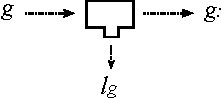
\includegraphics{images/new-label}}%
  \qquad\qquad
  \begin{minipage}{1.2in}%
    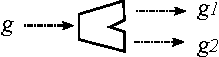
\includegraphics{images/split-gen}
  \end{minipage}%
  \caption{Graphical renderings of $new$ (left) and $split$ (right)}%
  \label{fig:new-and-split}%
\end{figure}



\subsubsection{Model for $new$ and $split$}

The conceptually simplest model of such generators
is one where labels produced are simply the strings of $:$, $1$ and $2$
that designate how the generator was produced from the original root.
For full clarity we show the model here using the full notation.
Both generators and labels are now represented as sequences of the three symbols
$:$, $1$ and $2$.
\RLEQNS{
  s \in LblSym &=& \setof{\texttt{:},\texttt{1},\texttt{2}}
\\ g \in GenSym &=& LblSym^*
\\ l \in Label &=& LblSym^*
\\ new(g) &\defs&  (g,g \cat \seqof{\texttt{:}})
\\ split(g) &\defs&  (g \cat \seqof{\texttt{1}},g \cat \seqof{\texttt{2}})
}
With this model we also get the following law:
For any generator expression $G$,
the following four sets are mutually disjoint:
\[
  \setof{\ell_G}
  \quad
  labs(G_{:})
  \quad
  labs(G_1)
  \quad
  labs(G_2)
  \qquad
  \elabel{labs-fully-disjoint}
\]
This is stronger than we require, but this is not a problem.
We also get three very significant benefits from this model/notation:
\begin{enumerate}
  \item
    It is very easy to decide if two generator expressions
    denote the same label---they do if and only if the expressions are the
    same, which in shorthand terms means the label sequences are the same.
  \item
    It is almost as easy to decide if two generator expressions produce
    disjoint labels.
    This occurs if and only if neither of the sequences of postfix operators
    involved are a prefix of the other.
    Or put differently, a generator's labels are a subset of another's
    iff its postfix sequence extends that of the other generator:
    \RLEQNS{
       labs(\g{\rho}) \subseteq labs(\g{\varrho}) &\equiv& \varrho \leq \rho
       & \elabel{prefix-lab-subset}
    }
    where $\leq$ is the sequence prefix relation.
  \item
    We refer to $g$ as the ``root'' in double quotes,
    because $g$ is not privileged in any way.
    If we substitute a different expression $G$ for $g$
    in the semantics of a construct,
    the behaviour is unchanged.
    In effect $g$ is like a ``base address'',
    with all the labels generated from $g$ being relative to it,
    and replacing $g$ by $G$ simply relocates it and the labels it generates.
    This is the basic mechanism used to construct the semantics
    of all the composite constructs in the language.
\end{enumerate}


\subsection{Label-Set Invariants}

The semantics we propose here depends on the careful management
of when specific labels are, or are not,
present in the global label-set $ls$.
We are looking at a situation where the semantics of any construct
requires associating unique labels with its entry and exit points,
as well as having a label generator provided for use with any sub-components
it might have.

So, from the perspective of any well-program $P$,
we have the following three (static) observation variables.
\RLEQNS{
   in, out &:& Lbl
\\ g &:& Gen
}
Key to the success of this semantics is a collection of label-set invariants
which characterise proper label-set contents,
which are preserved by all label-set manipulations performed
by our semantic definitions.

\subsubsection{Disjoint Labels (DL)}\label{sssec:disjoint-labels}

The first invariant we have is simply one that asserts,
for every construct, that $in$, $out$ and the labels of $g$
are all different
\footnote{The theory can be developed using only $g$ as a static observation,
and letting $\ell_g$ and $\ell_{g:}$ play the role of $in$ and $out$
respectively, in which case Disjoint Labels is automatically satisfied.
However, while this results in an entirely equivalent theory,
it is notationally much more obscure
with definitions and results that are harder to interpret and check.
}%
\RLEQNS{
   in \neq out &\land& \setof{in,out} \cap labs(g) = \emptyset
   & \ecite{Disjoint-Labels}
}



\subsubsection{Label Exclusivity (LE)}\label{sssec:label-exclusivity}

In addition to Disjoint Labels above,
which merely ensures distinctness of labels themselves,
we also need stronger invariants regarding which labels can, or cannot,
occur in the global label set at any one time.
There is not one such Label Exclusivity invariant,
but rather we have that each language construct defines it own
variation, in order to ensure that flow of control is correctly managed.

There is a general version of the invariant, as follows:
\RLEQNS{
   &&
   in \in  ls \implies (\setof{out} \cup labs(g))\cap ls = \emptyset
\\ &\land&
   (labs(g) \cap  ls \neq \emptyset) \implies \setof{in,out}\cap ls = \emptyset
\\ &\land&
   out \in ls \implies (\setof{in} \cup labs(g))\cap ls = \emptyset
   & \ecite{Exclusive-Labels}
}

We also more specific invariants, specific to each composite language construct.
We start with one of the simplest,
namely that used by sequential composition.
It asserts that any point in time,
only one of $in$, $\ell_g$ or $out$ can be present in $ls$:
\RLEQNS{
   &&
   in \in  ls \implies \setof{\ell_g,out}\cap ls = \emptyset
\\ &\land&
   \setof{\ell_g} \subseteq ls \implies \setof{in,out}\cap ls = \emptyset
\\ &\land&
   out \in ls \implies \setof{in,\ell_g}\cap ls = \emptyset
}
The most complex example is that for parallel composition.
Here we have four labels in addition to $in$ and $out$,
namely $\ell_{g1}$, $\ell_{g1:}$, $\ell_{g2}$, and $\ell_{g2:}$.
They should not occupy $ls$ at the same time as either $in $ or $out$,
but we also have that only one of the pair $(\ell_{g1},\ell_{g1:})$
can be present at the same time,
and the same must hold  for $(\ell_{g2},\ell_{g2:})$.
\RLEQNS{
   &&
   in \in ls
   \implies
   \setof{\ell_{g1},\ell_{g1:},\ell_{g2},\ell_{g2:},out}\cap ls = \emptyset
\\ &\land&
   \ell_{g1} \in ls \implies \setof{in,\ell_{g1:},out}\cap ls = \emptyset
\\ &\land&
   \ell_{g1:} \in ls \implies \setof{in,\ell_{g1},out}\cap ls = \emptyset
\\ &\land&
   \ell_{g2} \in ls \implies \setof{in,\ell_{g2:},out}\cap ls = \emptyset
\\ &\land&
   \ell_{g2:} \in ls \implies \setof{in,\ell_{g2},out}\cap ls = \emptyset
\\ &\land&
   out \in ls
   \implies
   \setof{in, \ell_{g1},\ell_{g1:},\ell_{g2},\ell_{g2:}}\cap ls = \emptyset
}
The precise motivation for these will be explained when the relevant
construct semantics are being described later.
For now we simply observe,
that these invariants are quite bulky and complex.



\subsubsection{Label-Set Invariant Notation}

First we shorten $labs(g)$ to just $g$ when this is clear from context,
i.e., a label-set, rather than a generator, is expected.

The Disjoint Labels invariant basically asserts
that a number of sets of labels are mutually disjoint.
We use the following shorthand, where the $L_i$ are label-sets,
\RLEQNS{
   \setof{L_1|L_2|\dots|L_n}
   &\defs&
   \forall_{i,j \in 1\dots n}
    @
    i \neq j \implies L_i \cap L_j = \emptyset
\\ \multicolumn{3}{c}{\elabel{short-disj-lbl}}
}
So we have an alternative definition of the Disjoint Labels invariant:
\RLEQNS{
 && \setof{in|g|out} & \elabel{Disjoint-Labels}
}

In a similar vein, we use a similar shorthand notation
for the Label Exclusivity invariants.
We use a shorthand,
whose easy cases can be formulated as follows:
\RLEQNS{
   ~[L_1|L_2|\dots|L_n]
   &\defs&
   \forall_{i,j \in 1\dots n}
    @
    i \neq j \implies
     ( L_i \cap ls \neq \emptyset \implies L_j \cap ls = \emptyset )
\\ \multicolumn{3}{c}{\elabel{short-lbl-exclusive}}
}
So the sequential composition Label Exclusivity invariant
is simply: $[in|\ell_g|out]$.
What needs to be kept in mind regarding this shorthand notation
is that $ls$ is mentioned under the hood,
and it is really all about what can be present in the global label-set
at any instant in time.

For parallel composition, we a little more complexity.
In shorthand it is expressed as
\[
   [in|(\ell_{g1}|\ell_{g1:}),(\ell_{g2}|\ell_{g2:})|out].
\]
It asserts at the top-level that $ls$
may contain only $in$, only $out$,
or only labels in $\ell_{g1},\ell_{g1:},\ell_{g2},\ell_{g2:}$.
In addition however, $\ell_{g1}$ and $\ell_{g1:}$ cannot occur together
and neither can $\ell_{g2}$ and $\ell_{g2:}$.

A more detailed and formal description of this way of describing
these invariants, in terms of an different abstract notation,
is presented in \S\ref{ssec:exclusive-lsat}.

\subsubsection{Properties of DL and LE}

Consider the following two generic examples:
\begin{enumerate}
  \item
    $DL_n = [L_1|L_2|\dots|L_n]$
    asserts that each $L_i$ is disjoint from any other.
  \item
    $LE_n = \{L_1|L_2|\dots|L_n\}$
    asserts that if elements one $L_i$ are in $ls$,
    then no elements from the others are.
\end{enumerate}

The ordering in either invariant is immaterial.
If $\rho$ is a permutation over $\setof{1\dots n}$ then
\RLEQNS{
   \{L_1|L_2|\dots|L_n\} &=& \{L_{\rho1}|L_{\rho2}|\dots|L_{\rho n}\}
   & \elabel{DL-perm}
\\ ~[L_1|L_2|\dots|L_n] &=& [L_{\rho1}|L_{\rho2}|\dots|L_{\rho n}]
   & \elabel{LE-perm}
}
Both invariants imply shorter versions of themselves:
\RLEQNS{
   \{\dots|L_{i-1}|L_i|L_{i+1}\dots\} &\implies& \{\dots|L_{i-1}|L_{i+1}\dots\}
   & \elabel{DL-drop}
\\ ~[\dots|L_{i-1}|L_i|L_{i+1}\dots] &\implies& [\dots|L_{i-1}|L_{i+1}\dots]
   & \elabel{LE-drop}
}
Both invariants imply versions with smaller sets:
\RLEQNS{
   S_i \subseteq L_i \land \{L_1|\dots|L_n\}
   &\implies& \{S_1|\dots|S_n\}
   & \elabel{DL-subset}
\\ S_i \subseteq L_i \land [L_1|\dots|L_n]
   &\implies& [S_1|\dots|S_n]
   & \elabel{DL-subset}
}
A key property shared by all LE invariants,
is that they are trivially satisfied by $ls = \emptyset$,
or if $ls$ only contains labels not mentioned in the invariant.
\RLEQNS{
   scope(LE_n) &\defs& L_1 \cup L_2 \cup \dots \cup L_n
\\ (ls = ls \setminus scope(LE_n)) &\implies& LE_n = \true
    & \elabel{LE-out-of-scope}
\\ ls = \emptyset &\implies& LE_n = \true
    & \elabel{LE-trivial}
}
There is no simple relationship between $DL_n$ and $LE_n$.
It is possible for one to be true when the other is false.
\begin{description}
  \item[DL true, LE false]
    $L_1 \cap L_2 = \emptyset \quad\land\quad (L_1 \cup L_2) \subseteq ls$.
  \item[DL false, LE true]
    $L_1 = L_2 \quad\land\quad L_1 \cap ls = \emptyset$
\end{description}

\section{Observations}\label{sec:observe}

Any UTP theory has to cleary define its \emph{alphabet},
that is, the set of observational variables that define
its domain of discourse.
The theory presented here is inspired by UTPP\cite{DBLP:conf/icfem/WoodcockH02}
and uses some of the observations presented there:
the values associated with all (shared) variables
are not mentioned individually, but instead are lumped together;
and we assume that all actions are labelled and that we can observe
the set of labels that are considered to be ``active''.
\begin{eqnarray}
   s, s' &:& State
\\ ls, ls' &:& \power Lbl
\end{eqnarray}
The theory in \cite{DBLP:conf/icfem/WoodcockH02} also uses $ok$ and $ok'$,
but these are not required here
---they can added in though as derived observations, if wanted.

The role of label-generators is rather different, however.
They will be used to generate labels for statements,
and we do not want these to change during the lifetime of the program.
We will also want to be able to refer in a general way to two key labels
associated with any language construct,
namely the label ($in$) that is used to enable the starting of a construct,
and the label ($out$) that is used to signal that the construct has just terminated.
\begin{eqnarray}
   in, out &:& Lbl
\\ g &:& Gen
\end{eqnarray}
These observations are \emph{static},
in that their values do not change during program execution.
Instead, these variables record context-sensitive information about
how a language construct is situated with respect to its ``neighbours'',
in a way that permits a compositional approach.
For details of how this works, see Section \ref{sec:composing}.



Our semantics is built upon basic atomic state-change
actions that modify global shared state $s$.
The concurrent flow of control is managed using a global dynamic label-set $ls$
and the association of two distinguished labels $in$ and $out$,
and a label generator $g$ with every language construct.

This brings us to an important distinction between the usual approach
taken by UTP regarding the distinction between syntax and semantics.
The usual approach,
inspired by the slogan ``programs are predicates''\cite{predprog,conf/mlpl/Hoare85},
is to treat syntax and semantics as the same thing.
A program's syntax is simply a shorthand notation for its semantics.
So, the program text \texttt{x := x+y} \emph{is} a predicate,
a shorthand for the more verbose $x' = x + y \land y' = y$
\footnote{Assuming \texttt{x} and \texttt{y} are the only variables}
.
in particular, the notation for sequential composition, $P ; Q$,
is a shorthand for
$\exists obs_m @ P[obs_m/obs'] \land Q[obs_m/obs]$,
where $obs$ ($obs'$) refers to all the before- (after-)observations.
This ``punning'' between syntax and semantics largely works for theories
of sequential programs or local-state concurrency,
mainly because sequences of code lead to simple semantic sequencing.
However, in global shared-variable concurrency,
code sequences get broken up by interference from parallel execution threads,
and there is no longer a simple correspondence between syntactical and semantic
sequencing.

Here we shall use the notation $P;Q$
to denote \emph{semantic} sequential composition,
which means that the execution of $P$ is immediately followed by the
execution of $Q$, without any intervening external interfence.
We define it as follows:
\begin{equation}
   P ; Q \defs \exists s_m, ls_m @ P[s_m,ls_m/s',ls'] \lor Q[s_m,ls_m/s,ls]
   \label{eqn:semantic-;}
\end{equation}
The key thing to note is that this definition makes no reference at all
to $g$, $in$ or $out$,
as these are static observations.
A desired consequence of this is that
substitutions $\gamma$ that
replace $g$, $in$ and/or $out$
by expressions that only involve the static variables,
will distribute through semantic sequential composition:
\begin{equation}
  (P ; Q)\gamma = (P\gamma) ; (Q\gamma)
\end{equation}

\section{Atomic Actions}\label{sec:atomic}

\section{Healthiness}\label{sec:health}


\subsubsection{Wheels-within-Wheels}\label{ssec:WwW}

The key intuition behind this compositional semantics was to take the
top-level $run$ function of the action-system based semantic model used in UTPP,
and drive it inwards to every level of the program.
The original $run$ can be defined in the context of this theory as
\[
  run(P) = ls := \setof{in} ; \lnot (out \in ls) * P
\]
However this failed to keep atomic components ``live''.
They could never be re-executed,
as would be required if they were within an iteration.
Instead it was realised that every construct (atomic and composite)
would have to be within an infinite loop.%
\RLEQNS{
    \true * P &\elabel{WWW-as-loop}
}%
This wrapping of the basic property in an infinite loop
would occur at every level of the program hierarchy,
hence the our use of the phrase ``Wheels within Wheels''
(WwW) to refer to this principle.

It should be noticed that this theory underwent
a large enumber of iterations before the WwW principle was finally
elucidated properly and shown to give the right results.
Earlier work in this area, reported in \cite{conf/tase/BMN16},
still had $run$ as shown above and was not fully compositional.
The number and complexity of the test calculations needed to debug,
develop and validate the theory presented in this paper
necessitated the develoment of a bespoke ``UTP Calculator''\cite{DBLP:conf/utp/Butterfield16}.

This bold step turns out to be remarkably effective,
with some quite counter-intuitive outcomes.
However it does depend on a specific tweak to the
definition of an atomic action.
In effect we define an atomic action
as placing a basic action inside such a loop,
but within a non-deterministic choice between it
and a \emph{stuttering} step, denoted by UTP's \emph{semantic} skip ($\Skip$):
\RLEQNS{
  \catom a &=& \true * (\Skip \lor A(in|a|out))
\\ \Skip &=& s'=s \land ls'=ls
}
A result of this is that this stuttering step gets
propagated up to enclosing composites,
so in effect we see $\true * C = \true * (\Skip\lor C)$
where $C$ is any predicate denoting the semantics of a command.
Given that our loop bodies always have such a disjunction,
it then becomes interesting to ask what this looks like:
\RLEQNS{
  \true * (\Skip \lor P) &=& \bigvee_{i \in \Nat} P^i
  & \elabel{loop-as-NDC}
}
We find that such a loop is equivalent to a non-deterministic
choice over the number of times that $P$ is repeated,
including zero.

We choose to \emph{define} the healthiness condition as
this large choice.
\RLEQNS{
   P^0 & \defs& \Skip           & \elabel{seq-0}
\\ P^{i+1} & \defs& P \seq P^i  & \elabel{seq-i-plus-1}
\\ \lhsWWW &\defs& \rhsWWW & \elabel{\lblWWW}
}
We note that $\WWW$ is monotonic and idempotent.

\subsection{Label-Set Invariants}


The semantics we propose here depends on the careful management
of when specific labels are, or are not,
present in the global label-set $ls$.
Key to the success of this semantics is a collection of label-set invariants
which characterise proper label-set contents,
which are preserved by all label-set manipulations performed
by our semantic definitions.
We have two kinds of invariants,
both of which are concerned with the mutual disjointness, in some sense,
of a collection of sets of labels.
We introduce some shorthand notations
to avoid excessively long predicates and expressions.
We use `$\mid$' as a seperator between things meant to be disjoint,
and commas to list subsets and/or set- elements that should be unioned together.
So the fragment $ A,b | M,N | x,Y $
is shorthand for the mutual disjointness of
$A \cup \setof a$ and $M \cup N$ and $\setof x \cup Y$.
To assert mutual set disjointness,
we use the following shorthand, where the $L_i$ are label-sets,
\RLEQNS{
   \setof{L_1|L_2|\dots|L_n}
   &\defs&
   \forall_{i,j \in 1\dots n}
    @
    i \neq j \implies L_i \cap L_j = \emptyset
\\ \multicolumn{3}{c}{\elabel{short-disj-lbl}}
}
We also want to assert that certain sets, necessarily mutually disjoint,
can never have any of their elements in the global label-set,
if any element from one of the other sets is present.
Again, we have a shorthand:
\RLEQNS{
   ~[L_1|L_2|\dots|L_n]
   &\defs&
   \forall_{i,j \in 1\dots n}
    @
    i \neq j \implies
     ( L_i \cap ls \neq \emptyset \implies L_j \cap ls = \emptyset )
\\ \multicolumn{3}{c}{\elabel{short-lbl-exclusive}}
}

The first invariant we have, Disjoint Labels ($DL$) is simply one that asserts,
for every construct, that $in$, $out$ and the labels of $g$
are all different.
\footnote{The theory can be developed using only $g$ as a static observation,
and letting $\ell_g$ and $\ell_{g:}$ play the role of $in$ and $out$
respectively, in which case Disjoint Labels is automatically satisfied.
However, while this results in an entirely equivalent theory,
it is notationally more obscure
making it harder to interpret and check.
}%
\RLEQNS{
   DL &\defs& \setof{in|labs(g)|out} & \elabel{Disjoint-Labels}
}
We shall simplify further by stating that in the shorthands presented
here that we use just simple $g$ to denote $labs(g)$,
so $DL$ can we written as $\{in|g|out\}$.
We also need stronger Label Exclusivity invariants,
regarding which labels can, or cannot,
occur in the global label set at any one time.
There is not one such invariant,
but rather we have that some language constructs may define their own
variation, in order to ensure that flow of control is correctly managed.

There is a general version of the invariant ($LE$) that holds
for all language constructs that asserts that any point in time,
only elements from of one of $in$, $labs(g)$ or $out$
can be present in $ls$ at any point in time:
\RLEQNS{
   LE &\defs&
   ~[in|g|out]
   & \ecite{Exclusive-Labels}
}
Note that we also just use a dash to make
the same assertion about the allowable contents of $ls'$
by simply writing $[in|g|out]'$.'

So, in summary, we have that every healthy predicate describing
a shared-variable concurrent program's behaviour is of the form $\WWW(C)$
for some predicate $C$ and also satisfies $DL$ and maintains $LE$.

\section{Command Semantics}\label{sec:semantics}

We present the full semantics of atomic commands first,
then describe an important classification of expressions and substitutions,
before describing the semantics of the four composite command forms.

\subsection{Atomic Commands}\label{ssec:atomic}

The atomic command $\catom a$ can be very simply expressed as basic action
with the addition of healthiness conditions:
\RLEQNS{
   \lhsW &\defs& DL \land LE \land \WWW(P) & \elabel{\lblW}
\\ \lhsCA &\defs& \rhsCA & \elabel{\lblCA}
}
Here we would expect that if $LE$ holds when this action starts,
i.e. when $in \in ls$ and it gets to run,
that $LE'$ should also hold, with $out \in ls'$.

\subsection{Grounded and Sound}

Given that we have a distinction between static observations ($g$, $in$, $out$),
and dynamic ones ($s,s',ls,ls'$) it is worth extending this distinction
to expressions and substitutions.
The reason for this is do with the fact that, by design,
semantic sequantial composition ignores the static variables.
An expression is ``ground'' if the only variables present are static.
A substitution is also deemed ``ground'',
if all the the replacement expressions are ground,
and the target variables are all static.
A desired consequence of this is that
ground substitutions $\gamma$
will distribute through semantic sequential composition,
semantic skip,
and both disjoint label-set notations
\RLEQNS{
   (P\seq Q)\gamma &=& P\gamma \seq Q\gamma  & \elabel{seq-gnd-distr}
\\ \Skip\gamma     &=& \Skip                 &\elabel{skip-gamma}
\\ ~\{L_1|\dots|L_n\}\gamma &=& \{L_1\gamma|\dots|L_n\gamma\}
& \elabel{DL-gamma-subst}
\\ ~[L_1|\dots|L_n]\gamma &=& [L_1\gamma|\dots|L_n\gamma]
& \elabel{LE-gamma-subst}
}
Groundness is not enough, we also require substitutions to be ``sound''
in the sense that they cannot transfrom a situation that satisfies $DL$
or $LE$ into one that does not.
A ground substitution $\varsigma$, of the form $[G,I,O/g,in,out]$ is \emph{sound}
if $\setof{I|G|O}$ holds.
We will see that all substitutions in the semantic definitions
below are sound, and that this is easy to check by inspection.


\subsection{Composing Actions}\label{ssec:composing}

The semantics of composite actions basically involves using the generator
to produce a suitable number of labels,
that are then used in zero or more ``control-flow'' actions
of the form $A(E|ii|N)$, where $ii$ is atomic skip that simply asserts $s'=s$.
The left-over generator is the split as required,
and then the components are ``connected'' into
the relevant new labels and generators using sound substitutions.
Finally the relevant healthiness conditions are supplied.
A key principle is to ensure that when any sub-component is ``active'',
that is, at least one of its labels is present in $ls$,
that none of the labels of the parent,
other than those explicitly shared with the sub-component,
are themsleves in $ls$.
This prevents a parent starting a spurious copy of a sub-component
while that sub-component is actually running.
The semantic definitions are listed in Fig. \ref{fig:composite-semantics}.
Careful inspection of all the substitutions present will confirm that they
are all sound.
\begin{figure}[t]
  \RLEQNS{
     \lhsSEQ &\defs& \rhsSEQ & \elabel{\lblSEQ}
  \\ \lhsPAR
     &\defs&
     \leftW \rhsaPAR \lor {}
     & \elabel\lblPAR
  \\&& \phW \rhsbPAR \lor {}
  \\&& \phW \rhscPAR \lor {}
  \\&& \phW \rhsdPAR \rghtW
  \\ \lhsNDC &\defs& \invNDC \land \rhsNDC & \elabel{\lblNDC}
  \\ \lhsSTAR
     &\defs&
     \leftW \rhsaSTAR \lor {}
     & \elabel\lblSTAR
  \\&& \phW \rhsbSTAR \lor {}
  \\&& \phW \rhscSTAR \lor {}
  \\&& \phW \rhsdSTAR \rghtW
  }\caption{Composite Semantics}
\label{fig:composite-semantics}
\end{figure}
Given that the invariant $LE$, which is $[in|labs(g)|out]$,
is part of the definition of $\W$,
then we have it statisfied, by definition, by any sub-components.
From the perspective of the parent composite, this means that $LE\varsigma$
also holds, where $\varsigma$ ranges over all the sound substitutions
used in the definition of the parent's semantics.
For example, for program sequential composition,
we not only assert $[in|g|out]$,
but can also infer $[in|\g{:1}|\ell_g]$
and $[\ell_g|\g{:2}|out]$.
Some constructs require a little more than just $DL$, $LE$ and the sound substitution
variants just discussed.
For example in program non-deterministic choice ($+$),
we need to insist that only one branch is taken, hence
the need to assert that if any label is present in $ls$ from one component
then none from the other are present.


In summary,
we have have predicate semantics for atomic and composite program
constructs,
in which everything at every level is wrapped in an infinite loop.
This seems to be completely counter-intuitive:
a program that consists of a single atomic action may wait
for a while while external interference rumbles on,
but eventually it should get ``scheduled'', perform its atomic action
and then effectively stop.
How is this consistent with looping forever?
To see the answer to this question,
it helps to consider such simple examples,
and this brings up the issue of \emph{calculation}.

\section{Calculations}\label{sec:calc}

This semantic theory was validated by a series of test calculations
done to ensure that it was making the right predications about program behaviour.
This typically involved taking small programs with a few atomic actions
and trying to simplify their semantic predicates
down to a non-deterministic choice of atomic action sequences.
Some of the calculations proved to be very long,
repetitive and tedious,
motivating the UTP-calculator development \cite{DBLP:conf/utp/Butterfield16}.

We shall start by sketching out a test calculation for $\catom a$,
where the objective is to reduce it down to a predicate involving
just basic atoms.
\RLEQNS{
  & & \lhsCA
\\&=& \rhsCA                                    & \elabel{\lblCA}
\\&=& DL \land LE \land \WWW(A(in|a|out))       & \elabel{\lblW}
\\&=& DL \land LE \land \bigvee_i A(in|a|out)^i & \elabel{\lblWWW}
}
At this point what remains is to compute $A(in|a|out)^i$ for $i \in \Nat$.
The cases of $i=0,1$ are straightforward.
Computing $i=2$ is easy:
\RLEQNS{
  &  & A(in|a|out) \seq A(in|a|out)     & \elabel{X-def}
\\&=& X(in|a|in|out) \seq X(in|a|in|out) &\elabel{X-then-X}
\\&=& \setof{in} \cap (\setof{in}\setminus\setof{out}) = \emptyset
      \land
      X(\dots) & \mbox{set theory}
\\&=& \false \land X(\dots)
}
We see that $A(in|a|out)^2 = \false$, and as $\false$ is a zero for
semantic sequential composition,
we can deduce that $A(in|a|out)^i = \false$ for all $i \geq 2$.
So our final result is
\begin{equation}
  \catom a = DL \land LE \land(\Skip \lor A(in|a|out))
\end{equation}
Ignoring the healthiness conditions,
this boils down to two possible observations we can make of $\catom a$:
either we observe suttering---no change in state or label-sets ($\Skip$)
or we see the complete execution of the underlyng basic action $A(in|a|out)$.

Test calculations for simple usage of most of the composites is essentially the
same.
One slight complication is that the contents of $\WWW$ in theses cases
is a disjunction of terms, rather than a single basic action,
so we first simplify these out, applying all substitutions,
to get a term $Q$ of the form ($\Skip \lor \textit{basic actions}$).
We need to compute $Q^i$ for $i \geq 2$,
and sequential composition distributes through disjunction,
so we obtain resulting terms of the same form,
by repeated application of law \elabel{X-then-X}.
A large number of these have results
with the set side-condition that evaluates to \false,
as per the $i=2$ example above---these terms vanish.
There are other terms produced that do not vanish,
but some of these can also be eliminated,
because their enabling set violates the Label Exclusivity invariant.
All remaining terms have the form $X(E|a|R|N)$,
and some of these can be immediately re-written to $A(E|a|N)$,
if $R=E$.
In every test calculation we have done
it turns out that the others, where $R\neq E$ can also be re-written,
because $LE$ says that none of $R \setminus E$ can be present in $ls$
when anything from $E$ is present,
so the removal of those labels is ineffective, as they are never present
when that action is enabled.
So, the outcome is that we get final results where every basic action
can be written in the $A$-form.
All of these aspects of these test calculations are supported by current
versions of the tool described in \cite{DBLP:conf/utp/Butterfield16}.
If there is no use of the iteration construct $(P^*)$,
then all calculations terminate because
there is always some $i$ for which $Q^i$ evaluates to \false.
Any use of the language iteration construct however
results in having terms for all values of $i$.

Some calculation results are shown in Fig. \ref{fig:calc-results}.
\begin{figure}[t]
\RLEQNS{
   \catom a \cseq \catom b
    &=&
    \Skip \lor A(in|a|\ell_g) \lor A(\ell_g|b|out) \lor A(in|ab|out)
\\ \catom a + \catom b
   &=& \Skip \lor A(in|ii|\ell_{g1}) \lor A(in|ii|\ell_{g2}) \lor A(\ell_{g1}|a|out)
\\ & &{} \lor A(\ell_{g2}|b|out) \lor A(in|a|out) \lor A(in|b|out)
\\ \catom a \parallel \catom b
   &=&
   \Skip \lor A(in|ii|\ell_{g1},\ell_{g2})
         \lor A(\ell_{g1:},\ell_{g2:}|ii|out)
         \lor A(\ell_{g1}|a|\ell_{g1:})
\\ & & {}
         \lor A(\ell_{g2}|b|\ell_{g2:})
         \lor A(in|a|\ell_{g1:},\ell_{g2})
         \lor A(in|b|\ell_{g2:},\ell_{g1})
\\ & & {}
         \lor A(\ell_{g1},\ell_{g2}|ba|\ell_{g1:},\ell_{g2:})
         \lor A(\ell_{g1},\ell_{g2}|ab|\ell_{g1:},\ell_{g2:})
\\ & & {}
         \lor A(\ell_{g2:},\ell_{g1}|a|out)
         \lor A(\ell_{g1:},\ell_{g2}|b|out)
         \lor A(in|ba|\ell_{g1:},\ell_{g2:})
\\ & & {}
         \lor A(in|ab|\ell_{g1:},\ell_{g2:})
         \lor A(\ell_{g1},\ell_{g2}|ba|out)
         \lor A(\ell_{g1},\ell_{g2}|ab|out)
\\ & & {}
         \lor A(in|ba|out)
         \lor A(in|ab|out)
}
\caption{
  Some Test Calculation Results.
  Here $ab$ ($ba$) is short for $a;b$ ($b;a$).
}
\label{fig:calc-results}
\end{figure}
If we look at the result for $\catom a \cseq \catom b$
we have $\Skip$, the stuttering step,
and $A(in|ab|out)$ which is
the complete exection of both actions without interference (mumbling),
and $A(in|a|\ell_g)$ that shows the execution of $a$, to an intermediate
point where $b$ has yet to occur.
These three observations are consistent with the idea that
our predicates are relations between a starting state and some subsequent
or final state.
However we also have action $A(\ell_g|b|out)$,
which is an observation that begins after action $a$ has already occured,
and just observes the behaviour of $b$ alone.
What has happened with this UTP theory of concurrency
is that it is now no longer insists that the ``before'' observation
is pinned to be the start of the program. Now we are able to observe program
behaviour that can both start and end at what are intermediate points
in the lifetime of the program.

If we look at $\catom a + \catom b$, we also explictly
see the control-flow ``decisions'',
such as $A(in|ii|\ell_{g1})$ where the decision to execute $a$ is made.
This will remove $in$ from $ls$ if it runs,
so disabling the other choice, denoted by $A(in|ii|\ell_{g2})$.
By contrast, in $\catom a\parallel \catom b$ the initially enabled
action is $A(in|ii|\ell_{g1},\ell_{g2})$, which activates both $a$ and $b$.
The control flow action $A(\ell_{g1:},\ell_{g2:}|ii|out)$ delays termination
until both atomic actions are done.

Finally,
we stress that the explicit inclusion of labels in the final results
is essential in order to ensure compositionality.
In \cite{conf/tase/BMN16} we had the explicit $run$ form,
and this reduced the semantics of $\catom a$ to $a$,
that of $\catom a + \catom b$ to $a \lor b$
and $\catom a \parallel \catom b$ to $ab\lor ba$.
While this looks cleaner, it has lost too much information,
and we cannot compose these further to get correct answers.
With the explcitly labelled semantics presented here for UTCP,
we can, for example, correctly compute $(\catom a \cseq \catom b) \parallel \catom c$
by replacing the first $\cseq$ term by its expansion
from Fig. \ref{fig:calc-results}.

\subsection{Future Work}\label{ssec:future}

While careful inspection and test calculations
give us a high level of confidence in the validity of our semantics,
we still need to demonstrate that the algebraic laws
of Concurrent Kleene Algebra\cite{}
can be derived form our semantics.
We also need to show how the standard operational semantics can be recovered.

Of particular interest is to explore the connection
between UTCP and rely-guarantee.
Given that we can explictly provide all atomic actions and their mumblings,
we see a good opportunity to explore how this can be exploited
to analyse how well one or more program steps satisfy their
guarantee obligation, given a reliable environment.

\section{Conclusions}\label{sec:conc}

We have presented a compositional, denotational UTP semantics
of shared-variable concurrency.
It is ``explicit'' in the sense that it can enumerate all the observations
that it is possible make of the program's own behaviour, in any time-slot.

The usefulness of this theory is that it is in a form that makes it very
easy for us to link it to other UTP theories about approaches to concurrency,
such as Rely-Guarantee\cite{DBLP:phd/ethos/Jones81,On-RG:vanStaden15},
Owicki-Gries\cite{DBLP:journals/acta/OwickiG76},
Concurrent Seperation Logic\cite{DBLP:journals/entcs/Brookes11},
all featured in the Views paper.
This is precisely because it is formulated as a before-after relation,
with the twist that before and after observations can occur at any time
during program execution, with the obvious proviso that
``before'' precedes ``after''.

\subsection{Future Work}\label{ssec:future}

While careful inspection and test calculations
give us a high level of confidence in the validity of our semantics,
we still need to demonstrate that the algebraic laws
of Concurrent Kleene Algebra\cite{}
can be derived form our semantics.
We also need to show how the standard operational semantics can be recovered.

Of particular interest is to explore the connection
between UTCP and rely-guarantee.
Given that we can explictly provide all atomic actions and their mumblings,
we see a good opportunity to explore how this can be exploited
to analyse how well one or more program steps satisfy their
guarantee obligation, given a reliable environment.



\bibliographystyle{splncs03}
\bibliography{UTCP-SBMF2017-MAIN}

\appendix

% \section{Denotations}\label{sec:denote}

\subsection{Overview}


Concurrent programs are a mix of control constructs ($\cseq,\parallel,+,\dots$)
and atomic actions $a$ that modify \emph{program state} $s$.
This is all that is visible to the programmer.



Our denotational UTP semantics
is inspired by that done for UTPP\cite{DBLP:conf/icfem/WoodcockH02},
itself based on a UTP theory of \emph{action systems}.
First, we add a new state component, not visible in the program text,
which is a set of labels ($ls$).
These labels are used to orchestrate the flow of control.
Given an atomic action $a$ that only knows about program state $s$,
we use notation $\catom a$ to describe a lifted version
of $a$ that takes account of the contents of the label-set $ls$.
In effect a lifted atomic state action is disabled until
a particular label is present in that set.
A disabled action does not modify the state any way
and simply monitors the label-set.
Once an action observes the presence/arrival of its label,
it then becomes active.
An active lifted action $\catom a$ atomically modifies the extended state as follows:
\begin{itemize}
  \item It makes the changes to $s$ as determined by its underlying action $a$.
  \item It removes the enabling label from the label-set.
  \item It adds in appropriate ``continuation'' labels to $ls$.
\end{itemize}
In \cite{DBLP:conf/icfem/WoodcockH02},
the language syntax required explicit (starting) labels
for every atomic state change action,
and these are used as lifted action enablers.
The continuation labels were taken to the the enabling labels
of whatever other actions occurred immediately after, in the program.
This means that the resulting semantics is not compositional.

The approach we adopt is to adopt the notion of \emph{label generators}
to create the labels, so ensuring they are unique,
but in such a way as make the generation a compositional process.
In addition we explicitly associate two labels with every program construct:
one that marks the entry into the construct,
and another that indicates the exit.

\subsubsection{On Notation}

We make liberal use of a number of shorthand notations,
largely to reduce expression size and clutter.
Typically these reduce the use of infix operators,
and in one notable case, collapse large conjunctions
of implications into a simple form with string visual cues.
Each shorthand is introduced by a subsection similar to this one.

\subsection{Label Generation}

INTRODUCE

\RLEQNS{
   g &:& Gen = \setof g  & \mbox{only one variable!}
\\ \ell &:& Gen \fun Lbl
\\ G \in Gen &::=&  g     & \mbox{the ``root'' generator}
\\           &\mid& G_{:} & \mbox{resulting generator after label produced}
\\           &\mid& G_1   & \mbox{first generator after generator split}
\\           &\mid& G_2   & \mbox{second generator after generator split}
\\ L \in Lbl &::=& \ell_G & \mbox{label produced by generator}
}
Note that our generator expression language has only one variable, $g$,
which denotes the ``root'' generator.
All generator expressions have the form $g$ followed by zero
or more uses of $:$, $1$ and $2$.
We say the  ``root'' generator because this notion is local to a
particular context, and we can relativise things by replacing $g$
by an arbitrary $G$ expression.
We define the notion of the set of labels produced by a generator,
which must satisfy the following laws:
\RLEQNS{
   labs &:& Gen \fun \power Lbl
\\ labs(G) &=& \setof{\ell_G} \cup labs(G_{:}) \cup labs(G_1) \cup labs(G_2)
  &\elabel{labs-def}
\\ \ell_G &\notin& labs(G_{:})
   &\elabel{labs-unique}
\\ \emptyset &=& labs(G_1) \cap labs(G_2)
  &\elabel{labs-split-disjoint}
}
The conceptually simplest model of such a generator
is one where labels are simply the strings of $:$, $1$ and $2$
that designate how its generator was produced from the root.
With this model we also get the following law:
For any generator expression $G$,
the following four sets are mutually disjoint:
\[
  \setof{\ell_G}
  \quad
  labs(G_{:})
  \quad
  labs(G_1)
  \quad
  labs(G_2)
  \qquad
  \elabel{labs-fully-disjoint}
\]

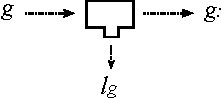
\includegraphics{images/new-label}

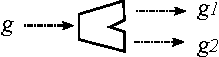
\includegraphics{images/split-gen}


\subsection{Observation Variables}

\begin{eqnarray*}
   s, s' &:& \mathcal S
\\ ls, ls' &:& \mathcal P (Lbl)
\\ g &:& Gen
\\ in, out &:& Lbl
\end{eqnarray*}
We assume a general notion of expressions ($e$)
and say that an expression $e$ is ``ground''
if it's free variables are limited to only $g$, $in$ and $out$.


\subsection{Label-Set Invariants}


We want to distinguish between disjointness only:
\[ \{ in | g | out \} \]
from disjointness with label-set exclusion:
\[ [ in | g | out ] \]

We want to be able to specify that certain combinations
of labels should never appear simultaneously
in the global label set ($ls$).
We do this by defining a label-set invariant $I$
which has alphabet $ls,in,out,g$.

We start by defining a general abstract way of specifying
sets with valid combinations
of values drawn from a parameter type $\tau$.
\RLEQNS{
   i \in I_\tau &::=& \tau   &  \mbox{can contain this value}
\\ &\mid& \otimes(i,\ldots,i) & \mbox{at most one of these allowed to contain}
\\ &\mid& \cup (i,\ldots,i) & \mbox{any of these allowed to contain}
}

We define what it means for an atomic action invocation
to satisfy an invariant parameterised on the label type ($Lbl$).
\RLEQNS{
  ls \textbf{ lsat } I \land A(E|a|N) &\implies& ls' \textbf{ lsat } I
}
We can re-formulate this as a following equivalent test:
\RLEQNS{
   A(E|a|N) \textbf{ sat } I_{Lbl}
   &\defs&
   E \textbf{ lsat } I_{Lbl} \land N \textbf{ lsat } I_{Lbl}
}
In effect we identify the occurrences of labels within this $I$-structure,
and then check the multiplicity constraints:
\RLEQNS{
   L \textbf{ lsat } I_{Lbl} &\defs& res=ok
\\ \textbf{where} && (res,\_) = occChk (occ_L I_{Lbl})
}
The $occ$ function takes a set $L$ of $\tau$ and an $I_\tau$ and returns a $I_\Bool$
that records if the corresponding element of $\tau$ is present in $L$.
\RLEQNS{
   occ &:& \power \tau \fun I_\tau \fun I_\Bool
\\ occ_L~\ell &\defs& \ell \in L
\\ occ_L~\otimes(i_1,\ldots,i_n)
   &\defs&
   \otimes(occ_L~i_1,\ldots,occ_L~i_n)
\\ occ_L~\cup(i_1,\ldots,i_n)
   &\defs&
   \cup(occ_L~i_1,\ldots,occ_L~i_n)
}
The $occChk$ function pattern matches across the boolean values to see if
constraints are satisfied.
The first component of the result is an overall ok/fail indicator,
while the second boolean component indicates if values are present
in any component.
\RLEQNS{
   occChk &:& I_\Bool \fun (\setof{ok,fail}\times \Bool)
\\ occChk(b) &\defs& (ok,b)
\\ occChk(\cup(i_1,\ldots,i_n))
   &\defs&
   (fail,\_),
   \textbf{ if }\exists j @ occChk(i_j) = (fail,\_)
\\ && (ok,b_1 \lor \dots \lor b_n),
   \textbf{ if }\forall j @ occChk(i_j) = (ok,b_j)
\\ occChk(\otimes(i_1,\ldots,i_n))
   &\defs&
   (fail,\_),
   \textbf{ if }\exists j @ occChk(i_j) = (fail,\_)
\\&& (fail,\_) \mbox{ if more than one $(ok,true)$}
\\&& (ok,false) \mbox{ if all are $(ok,false)$}
\\&& (ok,true) \mbox{ if  exactly one $(ok,true)$}
}
We note, as a consequence of the above definitions, that
\RLEQNS{
  \emptyset &  \textbf{lsat} &  I & \elabel{emp-lsat-I}
}
for any label-set invariant $I$.

We introduce a shorthand for invariants illustrated as follows.
\RLEQNS{
  ~ [ a,b,c | d,e | f ]
   &=&
   ls \textbf{ lsat } \otimes(\cup(a,b,c),\cup(d,e),f)
\\ ~[ a | (b|c),(d|e) | f ]
  &=&
  ls \textbf{ lsat } \otimes(a,\cup(\otimes(b,c),\otimes(d,e)),f)
}
In effect we make the involvement of $ls$ implicit,
and use bar ($|$) and comma ($,$) to replace $\otimes$ and $\cup$ respectively.
We also have a shorthand that just denotes
the non-intersecting nature of the arguments.
E.g.,
$\setof{A|B|C}$ asserts that $A$, $B$ and $C$ are mutually disjoint,
without any reference to $ls$ or any other set.

\subsubsection{Invariant Examples}

The following examples show how various instances of $ls \textbf{ lsat } I$
get expanded:
\RLEQNS{
   ~[in|out]
   &=&
   \setof{in} \cap \setof{out} = \emptyset
\\ &\land&
  \setof{in} \subseteq ls \implies \setof{out}\cap ls = \emptyset
\\ &\land&
  \setof{out} \subseteq ls \implies \setof{in}\cap ls = \emptyset
\\
\\ ~[in|\ell|out]
   &=&
   \setof{in} \cap \setof{\ell,out} = \emptyset
\\ &\land&
   \setof{\ell} \cap \setof{in,out} = \emptyset
\\ &\land&
   \setof{out} \cap \setof{in,\ell} = \emptyset
\\ &\land&
  \setof{in} \subseteq ls \implies \setof{\ell,out}\cap ls = \emptyset
\\ &\land&
  \setof{\ell} \subseteq ls \implies \setof{in,out}\cap ls = \emptyset
\\ &\land&
  \setof{out} \subseteq ls \implies \setof{in,\ell}\cap ls = \emptyset
\\
\\ ~[ a | (b|c),(d|e) | f ]
   &=&
   \setof{a} \cap \setof{b,c,d,e,f} = \emptyset
\\ &\land&
   \setof{b,c,d,e} \cap \setof{a,f} = \emptyset
\\ &\land&
   \setof{f} \cap \setof{a,b,c,d} = \emptyset
\\ &\land&
  \setof{a} \subseteq ls \implies \setof{b,c,d,e,f}\cap ls = \emptyset
\\ &\land&
  \setof{b,c,d,e} \subseteq ls \implies \setof{a,f}\cap ls = \emptyset
\\ &\land&
  \setof{f} \subseteq ls \implies \setof{a,b,c,d,e}\cap ls = \emptyset
\\ &\land&
   \setof{b} \cap \setof{c} = \emptyset
\\ &\land&
   \setof{d} \cap \setof{e} = \emptyset
\\ &\land&
  \setof{b} \subseteq ls \implies \setof{c}\cap ls = \emptyset
\\ &\land&
  \setof{c} \subseteq ls \implies \setof{b}\cap ls = \emptyset
\\ &\land&
  \setof{d} \subseteq ls \implies \setof{e}\cap ls = \emptyset
\\ &\land&
  \setof{e} \subseteq ls \implies \setof{d}\cap ls = \emptyset
}
Here one of $b$ or $c$ may occur in $ls$ along with one of  $d$ or $e$.
In this theory,
we use the label generators to ensure that the disjointness
conditions of the invariants are always true, by construction.

\subsubsection{Notation}

\RLEQNS{
   ls(\ell) &\defs& \ell \in ls
\\ ls(L) &\defs& L \subseteq ls
\\ ls(\B\ell) &\defs& \ell \notin ls
\\ ls(\B L) &\defs& L \cap ls = \emptyset
}



\subsection{``Standard'' UTP Predicates}

INTRODUCE

\RLEQNS{
   P \cond C Q
   &\defs&
   C \land P \lor \lnot C \land Q
   & \elabel{UTP-cond-def}
\\ \Skip
   &\defs&
   s'= s \land ls'=ls
   & \elabel{UTP-skip-def}
\\ P \seq Q
   &\defs& \exists s_m,ls_m \bullet
\\ && \qquad P[s_m,ls_m/s',ls'] \land Q[s_m,ls_m/s,ls]
   & \elabel{UTP-seq-def}
\\ C * P
   &=&
   P ; C * P \cond C \Skip
   & \elabel{UTP-loop-unroll}
}
We also define a specialised form of sequential composition
to be used when neither component refers to $ls$ or $ls'$,
and its unit:
\RLEQNS{
   P \seq_s Q
   &\defs&
   \exists s_m \bullet P[s_m/s'] \land Q[s_m/s]
   & \elabel{UTP-s-seq-def}
\\ ii &\defs& s'=s & \elabel{ii-def}
}
Note that if neither predicate mentions $ls$ or $ls'$
then the effect of $\seq$ and $\seq_s$ is the same.
We often omit the $s$ subscript when its use is clear from context.

\subsection{Healthiness Conditions}

\subsubsection{Disjoint Labels}

We have a general healthiness condition (Disjoint Labels) which asserts
that the labels associated with $in$, $out$ and $g$
are different:
\RLEQNS{
  \DL(P) &=& P \land in \neq out \land \setof{in,out} \cap labs(g) = \emptyset
}

\subsubsection{Wheels-within-Wheels}

The key intuition behind this compositional semantics was to take the
$run$ function of the action-system based semantic model used in UTPP,
and drive it inwards to every level of the program.
The original $run$ can be defined in the context of this theory as
\[
  run(P) = ls := \setof{in} ; \lnot (out \in ls) * P
\]
However this failed to keep atomic components ``live''.
They could never be re-executed,
as would be required if they were within an iteration.
Instead it was realised that every construct (atomic and composite)
would have to be within an infinite loop.
\RLEQNS{
   \W(P) &\defs& \true * P &\elabel{W-as-loop}
}
This bold step turns out to be remarkably effective,
with some quite counter-intuitive outcomes.
However it does depend on a specific tweak to the
definition of an atomic action.
In effect we define an atomic action
as placing a basic action inside such a loop,
but within a non-deterministic choice between it
and a \emph{stuttering} step, denoted by UTP skip:
\RLEQNS{
  \catom a &\defs& \W(\Skip \lor A(in|a|out))
}
A result of this is that this stuttering step gets
propagated up to enclosing composites,
so in effect we see $\W(C)=\W(\Skip\lor C)$
where $C$ is any predicate denoting the semantics of a command.
We give more details about this in the section on calculation (\S\ref{sec:calc}).
One key calculational advantage of this is that we can rewrite
the rhs of the definition of $\W$ as:
\RLEQNS{
   \W(P) &  =  & \bigvee_{i \in 0,\dots} \Skip \seq P^i &\elabel{W-as-NDC}
}%
We note explicitly here that, in effect,
our semantic model is based on unbounded non-determinism.

However, for iteration-free programs
we find that there is a finite $k$ such that $P^k = \false$,
in which case the non-determinism is bounded.
We get these finite results that seem very similar
to the results obtained by using $run$ above.
Using $run$ results in predicates that cannot be composed
to get composite behaviour.
However, using $\W$ results in a slight variation,
which is composable!
What turns out to be crucial
to this outcome is the explicit stuttering option in the infinite loop.

\subsubsection{Mumble Closure}

A program's semantics includes all its mumblings,
and so should be unchanged if sequentially composed with itself
using \emph{UTP} sequential composition:
\RLEQNS{
   P \seq P &=& P  & \eref{mumble-closure}
}

\subsection{UTP Denotational Semantics}

INTRODUCE

We present each construct individually,
with full diagrams for each \dots



\subsubsection{Basic Action}

Basic Action $A(E|a|N)$ is enabled when all the labels in $E$
are present in the global label-set
and atomic action $a$ does not evaluate to $\false$
in the current program state.
If so enabled,  it performs action $a$, removes the labels in $E$
from the label-set, and adds in those in $N$.
\RLEQNS{
   A(E|a|N)
   &\defs&
   ls(E) \land a \land ls'=(ls\setminus E) \cup N
   & \elabel{A-def}
}




\newpage
\subsubsection{Atomic Action}


\includegraphics{images/atomic-action}
\RLEQNS{
  \catom a
  &\defs& \DL(\W(\Skip \lor A(in|a|out))) & \elabel{sem:atomic}
\\ &=&  [in|out] \land (\Skip \lor A(in|a|out))
        & \elabel{nf-atomic}
}

Invariant Preservation:
\RLEQNS{
   [in|out]\gamma \land A(in|a|out)\gamma &\implies& [in|out]'\gamma
   & \elabel{atom-inv-ok}
}

\subsubsection{Guarded Atomic Action}
In effect there is no real difference between $c \pgrd a$
and $\true \pgrd (c \land a)$,
so in fact we don't need guarded actions as basic.
This is an advantage of treating the atomic action as a relational predicate
on state.

\RLEQNS{
 c \pgrd a &\defs& \catom{c \land a}  &\elabel{sem:pgrd}
}


\subsubsection{Skip}

\RLEQNS{
   ii     &\defs& s'=s
\\ \cskip &\defs& \catom{ii}  &\elabel{sem:skip}
\\  &=&  [in|out] \land (\Skip \lor A(in|ii|out))
    &\elabel{nf-skip}
}

\newpage
\subsubsection{Sequential Composition}

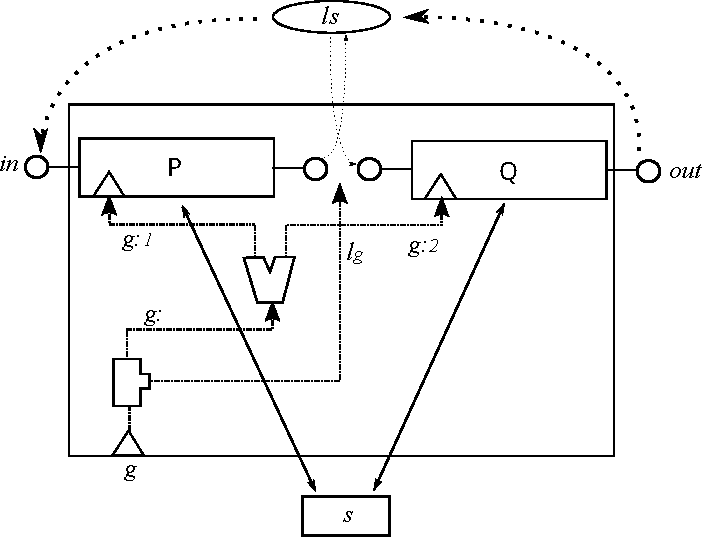
\includegraphics{images/seq-comp-actual}

\RLEQNS{
   P \cseq Q
   &\defs&
   [in|\ell_g|out]\land \W(P[g_{:1},\ell_g/g,out] \lor Q[g_{:2},\ell_g/g,in])
   & \elabel{sem:seq}
}

If $A$ actions in $P$ and $Q$ preserve the invariant,
then so does their composition.
This is immediate by the ground/sound substitution independence
of invariant preservation.



\newpage
\subsubsection{Parallel Composition}

\RLEQNS{
   P \parallel Q
   &\defs&
   [in|(\ell_{g1}|\ell_{g1:}),(\ell_{g2}|\ell_{g2:})|out] \land {}
   & \elabel{sem:par}
\\&& \W(\quad\phlor A(in|ii|\ell_{g1},\ell_{g2})
\\ && \qquad {}\lor
   P[g_{1::},\ell_{g1},\ell_{g1:}/g,in,out]
\\ && \qquad {}\lor
    Q[g_{2::},\ell_{g2},\ell_{g2:}/g,in,out]
\\ && \qquad {}\lor
   A(\ell_{g1:},\ell_{g2:}|ii|out)~)
}


\includegraphics{images/parallel-label-gen}

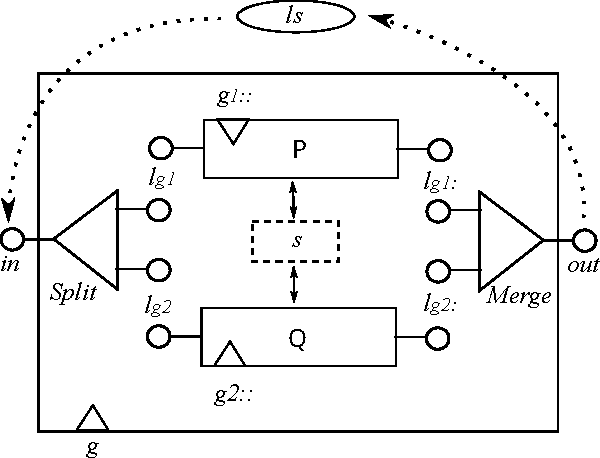
\includegraphics{images/par-comp-actual}


\newpage
\subsubsection{Nondeterministic Choice}

\RLEQNS{
   P + Q
   &\defs&
   [in|\ell_{g1}|\ell_{g2}|out] \land {}
   & \elabel{sem:NDC}
\\ && \W(\quad {}\phlor A(in|ii|\ell_{g1})
\\ && \qquad {} \lor
                     A(in|ii|\ell_{g2})
\\ && \qquad {} \lor
   P[g_{1:},\ell_{g1}/g,in]
\\ && \qquad {} \lor
   Q[g_{2:},\ell_{g2}/g,in]~)
}

\subsubsection{Nondeterministic Loop}


\RLEQNS{
   P^*
   &\defs&
   [in|\ell_g|out] \land {}
   & \elabel{sem:star}
\\ && \W(\quad  \phlor A(in|ii|out)
\\ && \qquad {}\lor A(in|ii|\ell_g)
\\ && \qquad {}\lor P[g_{:},\ell_g,in/g,in,out]~)
}

\newpage
\subsubsection{Conditional Choice}

\RLEQNS{
   P \dcond c Q
   &\defs&
   [in|\ell_{g1}|\ell_{g2}|out] \land {}
   & \elabel{sem:cond}
\\ && \W(\quad {}\phlor A(in|c \land ii|\ell_{g1})
\\ && \qquad {} \lor
                     A(in|\lnot c \land ii|\ell_{g2})
\\ && \qquad {} \lor
   P[g_{1:},\ell_{g1}/g,in]
\\ && \qquad {} \lor
   Q[g_{2:},\ell_{g2}/g,in]~)
}


\includegraphics{images/conditional-actual}

\newpage
\subsubsection{Conditional Loop}


\RLEQNS{
   c \ddo P
   &\defs&
   [in|\ell_g|out] \land {}
   & \elabel{sem:iter}
\\ && \W(\quad  \phlor A(in|\lnot c \land ii|out)
\\ && \qquad {}\lor A(in|c \land ii|\ell_g)
\\ && \qquad {}\lor P[g_{:},\ell_g,in/g,in,out]~)
}

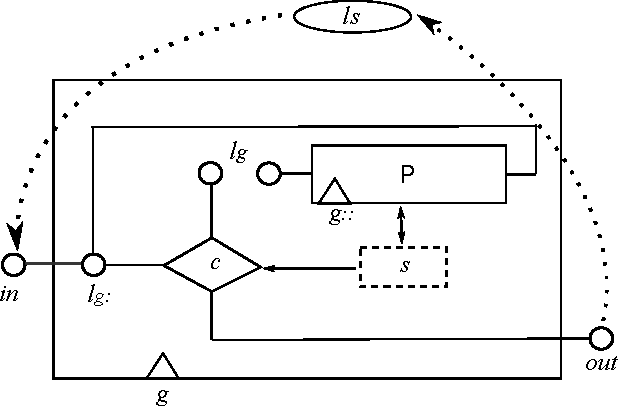
\includegraphics{images/iteration-actual}

\newpage
\subsection{Essential Properties?}

The first key property is that every instance of $A$
in the semantics preserves the invariant.

Looking forward we will want some key algebraic properties:
\RLEQNS{
   ~[S_1|\dots|S_n]
   &=&
   [S_{\rho(1)}|\dots|S_{\rho(n)}]
\\ && \rho \textrm{ a permutation of } 1\dots n
\\ ~[S_1|\dots|S_i|S_{i+1}|\dots|S_n]
   &\implies&
   [S_1|\dots|S_i]
   ,\quad i > 1 &\elabel{I-subsumption}
\\ ~[S_1|\dots|S_n]\gamma &=& [S_1\gamma|\dots|S_n\gamma]
   & \elabel{I-gamma-subst}
\\ A(E|a|N)\gamma &=& A(E\gamma|a|N\gamma)
\\ A(E|a|N) \textbf{ sat } I
   &=&
   A(E|a|N)\gamma \textbf{ sat } I\gamma
   , \quad \mbox{arbitrary }\gamma
\\ ((ls\setminus R)\cup A)(S)
   &=&
   ls(F(R,A,S)) \land P(R,A,S)
\\ \Skip \seq P &=~P~=& P \seq \Skip
\\ (P\seq Q)\gamma &=& P\gamma \seq Q\gamma  & \elabel{seq-gnd-distr}
\\ \Skip\gamma &=& \Skip
\\ \W(P)  && \textrm{monotonic in } P
\\ \W(\W(P)) &=& \W(P) & ?
\\ \W(\W(\Skip \lor P)) &=& \W(\Skip \lor P)
\\ \W(\Skip \lor P) &=& \bigvee_{i \in 0,\dots} \Skip \seq P^i
   & \elabel{W-as-NDC}
\\ \W(P)\gamma &=& \W(P\gamma) & \elabel{W-gamma-subst}
\\ \W(\Skip \lor P) &=& \Skip \lor \W(\Skip \lor P)
\\ I \land \W(P) &=& \W(I \land P) & \elabel{I-W-distr}
}

When $P\gamma$ executes:
\begin{description}
  \item[\elabel{P-removes-in}]
    it will remove $in\gamma$ from $ls$ at some point;
  \item[\elabel{P-removes-g}]
    the only other labels it removes are in $labs(g\gamma)$;
  \item[\elabel{P-adds-out}]
    it adds $out\gamma$ into $ls$ at some point;
  \item[\elabel{P-adds-g}]
    the only other labels it adds are in $labs(g\gamma)$;
  \item[\elabel{P-ignores-rest}]
    and its behaviour is not affected by any label not
    in
    \\$\setof{in\gamma,out\gamma} \cup labs(g\gamma)$.
\end{description}
We can summarise this as follows:
\begin{itemize}
  \item $P\gamma$ actions are enabled by labels in $in\gamma,g\gamma$
  \item $P\gamma$ actions enable actions enabled by $g\gamma,out\gamma$
  \item Remember that the following invariant holds: $[in\gamma|g\gamma|out\gamma]$
\end{itemize}




\newpage
\subsection{Miscellaneous}

Most of this stuff should end up,
if required,
in a Proofs/Justification appendix.

\subsubsection{Semantic Substitutions List}

It can be informative to see the invariants grouped with
the relevant actions and substitutions.
\RLEQNS{
   ~[in|out]
   && A(in|a|out)
\\ && id
\\
\\ ~[in|\ell_g|out]
   && [g_{:1},\ell_g/g,out]
\\ && [g_{:2},\ell_g/g,in]
\\
\\ ~[in|(\ell_{g1}|\ell_{g1:}),(\ell_{g2}|\ell_{g2:})|out]
   && A(in|ii|\ell_{g1},\ell_{g2})
\\ && A(\ell_{g1:},\ell_{g2:}|ii|out)
\\ && [g_{1::},\ell_{g1},\ell_{g1:}/g,in,out]
\\ && [g_{2::},\ell_{g2},\ell_{g2:}/g,in,out]
\\
\\ ~[in|\ell_{g1}|\ell_{g2}|out]
   && A(in|ii|\ell_{g1})
\\ && A(in|ii|\ell_{g2})
\\ && [g_{1:},\ell_{g1}/g,in]
\\ && [g_{2:},\ell_{g2}/g,in]
\\
\\ ~[in|\ell_g|out]
   && A(in|ii|out)
\\ && A(in|ii|\ell_g)
\\ && P[g_{:},\ell_g,in/g,in,out]
\\
\\ ~[in|\ell_{g1}|\ell_{g2}|out]
   && A(in|c \land ii|\ell_{g1})
\\ && A(in|\lnot c \land ii|\ell_{g2})
\\ && [g_{1:},\ell_{g1}/g,in]
\\ && [g_{2:},\ell_{g2}/g,in]
\\
\\ ~[in|\ell_g|out]
\\ && A(in|\lnot c \land ii|out)
\\ && A(in|c \land ii|\ell_g)
\\ && [g_{:},\ell_g,in/g,in,out]
}

\subsubsection{Nested Invariants}

For each composite,
we show how its component substitutions affect their invariants
and any entailment relationships that arise.
We don't show the conditional variants of choice and iteration
because their invariants and substitutions are the same as those
in the corresponding non-deterministic constructs.

Semantics Reminder:
\RLEQNS{
  \catom a
  &\defs& [in|out] \land \W(\Skip \lor A(in|a|out))
\\ P \cseq Q
   &\defs&
   [in|\ell_g|out]\land \W(P[g_{:1},\ell_g/g,out] \lor Q[g_{:2},\ell_g/g,in])
\\ P \parallel Q
   &\defs&
   [in|(\ell_{g1}|\ell_{g1:}),(\ell_{g2}|\ell_{g2:})|out] \land {}
\\&& \W(\quad\phlor A(in|ii|\ell_{g1},\ell_{g2})
\\ && \qquad {}\lor
   P[g_{1::},\ell_{g1},\ell_{g1:}/g,in,out]
\\ && \qquad {}\lor
    Q[g_{2::},\ell_{g2},\ell_{g2:}/g,in,out]
\\ && \qquad {}\lor
   A(\ell_{g1:},\ell_{g2:}|ii|out)~)
\\ P + Q
   &\defs&
   [in|\ell_{g1}|\ell_{g2}|out] \land {}
\\ && \W(\quad {}\phlor A(in|ii|\ell_{g1})
\\ && \qquad {} \lor
                     A(in|ii|\ell_{g2})
\\ && \qquad {} \lor
   P[g_{1:},\ell_{g1}/g,in]
\\ && \qquad {} \lor
   Q[g_{2:},\ell_{g2}/g,in]~)
\\ P^*
   &\defs&
   [in|\ell_g|out] \land {}
\\ && \W(\quad  \phlor A(in|ii|out)
\\ && \qquad {}\lor A(in|ii|\ell_g)
\\ && \qquad {}\lor P[g_{:},\ell_g,in/g,in,out]~)
}


\paragraph{Sequential Composition}

\begin{description}
  \item[Invariant]
    $[in|\ell_g|out]$
  \item[Substitutions]
    $[g_{:1},\ell_g/g,out]$ and $[g_{:2},\ell_g/g,in]$
  \item[Component Invariants]
    $$\begin{array}{|l|c|c|}
    \hline
      \mbox{Type} & \mbox{as }P & \mbox{as }Q
    \\\hline
      \catom\_ & [in|\ell_g] & [\ell_g|out]
    \\\hline
       \_\cseq\_& [in|\ell_{g:1}|\ell_g] & [\ell_g|\ell_{g:2}|out]
    \\\hline
       \_\parallel\_
       & [in|(\ell_{g:11}|\ell_{g:11:}),(\ell_{g:12}|\ell_{g:12:})|\ell_g]
       & [\ell_g|(\ell_{g:21}|\ell_{g:21:}),(\ell_{g:22}|\ell_{g:22:})|out]
    \\\hline
    \end{array}$$
\end{description}
Hmmm \dots, no simple relationship is emerging.

% \section{Semantic Calculations}\label{sec:calc}

\textbf{SHOULD COMPUTE PARTIAL NORMAL FORMS
FOR COMPOSTITES}

\subsection{Composing $A$s}\label{ssec:comp-A}

We have a problem in that actions defined using $A(\dots)$
are not closed under standard UTP sequential composition (\eref{UTP-seq-def}).
We need a more general form,
where the labels removed are not necessarily
exactly those that had to be present to enable the action.
We call this eXtended atomic action $X$ and it is defined as follows:
\RLEQNS{
   X(E|a|R|A)
   &\defs&
   ls(E) \land s' \in \sem a s \land ls' = (ls \setminus R) \cup A
   & \elabel{X-def}
}
We can then re-define $A$ in terms of $X$:
\RLEQNS{
   A(E|a|N)
   &=&
   X(E|a|E|N)
   & \elabel{A-alt-def}
}
The key law is one regarding sequentially composing $X$s:
\RLEQNS{
   \lefteqn{X(E_1|a|R_1|A_1) ; X(E_2|b|R_2|A_2)} &&& \elabel{X-then-X}
\\ &=& (E_2\setminus A_1) \cap R_1 = \emptyset
\\ &\land&
   X(E_1 \cup (E_2\setminus A_1)
       |a\seq b
       |R_1 \cup R_2
       |(A_1 \setminus R_2) \cup  A_2)
}
The condition $(E_2\setminus A_1) \cap R_1 = \emptyset$
characterises all those cases were the second $X$ is enabled
immediately after the first $X$ terminates
(i.e., without any outside interference).

\textbf{ANOTHER IMPORTANT LAW:}
If $(E_1 \cup N_1) \cap (E_2 \cup N_2)$, then
\[
  A(E_1|a|N_1) \seq A(E_2|b|N_2)
  =
  A(E_1\cup E_2|a\seq b|N_1\cup N_2)
\]
(and vice-versa)!

\subsection{Normal Form}\label{sec:normal-form}

All the semantics above have an invariant $I_P$,
zero or more atomic actions ($A_i$),
plus zero or more language sub-component predicates ($P_j$)
assembled into a predicate of the form:
\[
  I_P
  \land
  \W( A_1 \lor \dots \lor A_m
     \lor
     P_1\sigma_1 \lor \dots \lor P_n\sigma_n )
\]
where each $\sigma_i = [G_i,I_i,O_i/g,in,out]$,
with all $G_i$, $I_i$ and $O_i$ being ground
and satisfying the invariant $[I_i|labs(G_i)|O_i]$.

\subsubsection{Stuttering Propagates Up}

We show that for any predicate $P$ resulting from the
semantics applied to a program,
that the stuttering on such a predicate propagates up:
\RLEQNS{
   P &=& \Skip \lor P
}



\subsubsection{Nondeterministic Iteration}

Given that we have,
for predicates $P$ used in program semantic definitions,
that
\[
  \W(P) = \bigvee_{i \in 0\dots} \Skip \seq P^i
\]
we find that the following outcomes result:
\begin{enumerate}
  \item
    Every program $P$ can be transformed,
    in principle at least,
    to the form
    \[
      I_P \land \Skip
      \lor
      \bigvee_{n \in 0\dots}  (I_P \land I_n \land X(E_n|a_n|R_n|A_n) \land S_n)
    \]
    for suitable choices of $I_n$, $E_n$, $a_n$, $R_n$, $A_n$ and $S_n$,
    depending on $P$.
    In particular, we find that the $E_n$ and $A_n$ all satisfy the relevant
    label-set invariants.
  \item
    For any complete program that does not use iteration constructs,
    this expansion is finite.
  \item
    For any complete program the $S_n$
    term in $X(E_n|a_n|R_n|A_n) \land S_n$
    is a ground-expression, and is statically decidable as $\true$ or $\false$.
    If $\true$, we find that the above term
    can be be simplified to one of the form $A(E_n|a_n|A_n)$.
    We do not prove this, but note that we have observed it as a result
    of test calculations and these lead us to believe it is true in general.
\end{enumerate}
\RLEQNS{
   P
   &=&
   I_P \land \Skip
      \lor
      \bigvee_{n \in 0\dots}
      (I_P \land I_n \land X(E_n|a_n|R_n|A_n) \land S_n)
   & \elabel{UTCP-NF}
}
This can be shown by an inductive argument over the language syntax,
noting that the sequential composition of two such forms
can itself be transformed into such a form.
In effect this defines a \emph{normal form} for our semantics.


An important law we shall require is that the UTP sequential
composition of two normal forms can itself be expressed
as such a normal form:
\RLEQNS{
   I \land (\Skip\lor\bigvee A_i) \seq J \land (\Skip\lor\bigvee B_j)
   &=&
   I \land J \land (\Skip\lor\bigvee (A_i \seq B_j))
   &\elabel{nf-seq}
}
This is an easy result of the fact that $\seq$ distributes through $\lor$,
and $\Skip$ is a unit for it as well.


\subsection{Normal Form Results for Atomic components}

We now present the results of calculations of normal forms for every language
construct, given atomic sub-components,
and the generic case.

For ease of reading in the former,
we display the invariant $I$ on the first line,
followed by the list of $A(\dots)$ disjuncts, perhaps several on a line,
as follows
\RLEQNS{
   res &=& I
\\ && A(E_1|a_1|N_1) \quad A(E_1|a_2|N_2)) \quad \dots
}
We omit parentheses, logical operators, and the ever-present $\Skip$.
In general we try to put all the single atomic steps on the first line,
with all the mumblings on lower lines.
Here we also just write $a$ instead of $\catom a$,
for brevity.

In the latter generic case we  \emph{\dots to be determined \dots}

\subsubsection{Atomic Actions}
\RLEQNS{
   a &=& [in|out]
\\ && A(in|a|out) & \elabel{NF:atomic-a}
\\
\\ \cskip &=& [in|out]
\\ && A(in|ii|out) & \elabel{NF-skip}
}

\subsubsection{Sequential Composition}

With atomic components:
\RLEQNS{
   a \cseq b
   &=& [in|\ell_g|out]
\\ && A(in|a|\ell_g)\quad  A(\ell_g|b|out)
\\ && A(in|a\seq b|out)
}

With generic components:
\RLEQNS{
   P \cseq Q
   &=& [in|\ell_g|out]
\\ && A(in|a|\ell_g)\quad  A(\ell_g|b|out)
\\ && A(in|a\seq b|out)
}


\subsubsection{Non-deterministic Choice}
\RLEQNS{
   a + b
   &=& [in|\ell_{g1}|\ell_{g2}|out]
\\ &&  A(in|ii|\ell_{g1}) \quad A(in|ii|\ell_{g2})
       \quad
       A(\ell_{g1}|a|out) \quad A(\ell_{g2}|b|out)
\\&& A(in|a|out) \quad A(in|b|out)
}


\subsubsection{Parallel Composition}
Here $\#n$ denotes mumblings of length $n$.
\RLEQNS{
   a \parallel b
   &=& [in\mid([\ell_{g1}|\ell_{g1:}],[\ell_{g2}|\ell_{g2:}])\mid out]
\\ &&  A(in|ii|\ell_{g1},\ell_{g2})
       \quad
       A(\ell_{g1:},\ell_{g2:}|ii|out)
       \quad
       A(\ell_{g1}|a|\ell_{g1:})
       \quad
       A(\ell_{g2}|b|\ell_{g2:}) &
\\ && A(in|a|\ell_{g1:},\ell_{g2})
      \quad
      A(\ell_{g1},\ell_{g2}|b;a|\ell_{g1:},\ell_{g2:})
      \quad
      A(in|b|\ell_{g2:},\ell_{g1}) & \#2
\\ && A(\ell_{g1},\ell_{g2}|a ; b|\ell_{g1:},\ell_{g2:})
      \quad
      A(\ell_{g2:},\ell_{g1}|a|out)
      \quad
      A(\ell_{g1:},\ell_{g2}|b|out) & \#2
\\ && A(in|b;a|\ell_{g1:},\ell_{g2:})
      \quad
      A(in|a;b|\ell_{g1:},\ell_{g2:}) & \#3
\\ && A(\ell_{g1},\ell_{g2}|b;a|out)
      \quad
      A(\ell_{g1},\ell_{g2}|a;b|out) & \#3
\\ && A(in|b;a|out)
      \quad
      A(in|a;b|out) & \#4
}

\subsubsection{Non-deterministic Iteration}
The actions that denote a terminating
run with zero or more complete iterations
are \textbf{emboldended} below.
\RLEQNS{
   a^*
   &=& [in|\ell_g|out]
\\ &&  \mathbf{A(in|ii|out)} \quad A(in|ii|\ell_g) \quad A(\ell_g|a|in)
\\ &&  A(\ell_g|a|out) \quad A(\ell_g|a|\ell_g) \quad A(in|a|in)         &\#2
\\ &&  \mathbf{A(in|a|out)} \quad A(in|a|\ell_g) \quad A(\ell_g|a^2|in)  &\#3
\\ &&  A(\ell_g|a^2|out) \quad A(\ell_g|a^2|\ell_g) \quad A(in|a^2|in)   &\#4
\\ &&  \mathbf{A(in|a^2|out)} \quad A(in|a^2|\ell_g) \quad A(\ell_g|a^3|in) &\#5
\\ &&  A(\ell_g|a^3|out) \quad A(\ell_g|a^3|\ell_g) \quad A(in|a^3|in) &\#6
\\ && \vdots & \#7\dots
}
An obvious recurrent pattern (based on mumbling depth) has emerged:
\RLEQNS{
   &&  \mathbf{A(in|a^n|out)} \quad A(in|a^n|\ell_g) \quad A(\ell_g|a^{n+1}|in) &\#2n+1
\\ &&  A(\ell_g|a^{n+1}|out) \quad A(\ell_g|a^{n+1}|\ell_g) \quad A(in|a^{n+1}|in) &\#2n+2
}
We can also identify a pattern based on number of $a$s performed:
\RLEQNS{
   \alpha_0 && \mathbf{A(in|ii|out)} \quad A(in|ii|\ell_g)
\\ \alpha_1 && A(\ell_g|a|in) \quad A(\ell_g|a|out) \quad A(\ell_g|a|\ell_g) \quad A(in|a|in)
\\          && \mathbf{A(in|a|out)} \quad A(in|a|\ell_g)
\\ \alpha_2 && A(\ell_g|a^2|in) \quad A(\ell_g|a^2|out) \quad A(\ell_g|a^2|\ell_g) \quad A(in|a^2|in)
\\          && \mathbf{A(in|a^2|out)} \quad A(in|a^2|\ell_g)
\\
\\ \alpha_n && A(\ell_g|a^n|in) \quad A(\ell_g|a^n|out) \quad A(\ell_g|a^n|\ell_g) \quad A(in|a^n|in)
\\          && \mathbf{A(in|a^n|out)} \quad A(in|a^n|\ell_g)
}


\newpage
\subsection{Essential Properties?}

\RLEQNS{
   X(E|a|R|A)\gamma &=& X(E\gamma|a|R\gamma|A\gamma)
   & \elabel{X-gnd-subs}
\\ (\bigvee_n X_n)^2
   &=& \bigvee_{n_1,n_2} X_{n_1} \seq X_{n_2}
   & \elabel{NF-squared}
\\ (\bigvee_p Y_p \lor \bigvee_q Z_q)^2
     &=& \bigvee_{p_1,p_2}  (Y_{p_1} \seq Y_{p_2})
\\&\lor& \bigvee_{q_1,q_2}  (Z_{q_1} \seq Z_{q_2})
\\&\lor& \bigvee_{p,q}  (Y_p \seq Z_q)
\\&\lor& \bigvee_{q,p}  (Z_q \seq Y_p)
  & \elabel{NF+NF-squared}
\\ &=& \bigvee_r X_r,\textrm{ for appropriate } r
  & \elabel{NF-squared-alt}
\\ (\bigvee_p Y_p \lor \bigvee_q Z_q)^n
     &=& \bigvee_r X_r,\textrm{ for appropriate } r
  & \elabel{NF-powered}
\\ \W(\Skip \lor \bigvee_p Y_p \lor \bigvee_q Z_q)
     &=& \bigvee_r X_r,\textrm{ for appropriate } r
  & \elabel{W-of-NDC-is-NF}
}
Add in X-then-X and related properties.

Nice to have:
the combined invariants ensure that the normal form
has the form:
\[
  P = \bigvee_n A(E_n|a_n|N+n)  \qquad \elabel{NF-only-As}
\]
Is this the case?

\subsubsection{STOP PRESS! $P^2=P$ ?}

The semantics of a program $P$
contains a stuttering step $\Skip$,
all the single atomic actions $A(\dots)$,
and all the feasible mumblings
$X(\dots) = A(\dots) \seq A(\dots) \seq \dots \seq A(\dots)$.
Calculations for law $\cskip\cseq P = P$ suggest the following conjecture:
\begin{center}
\fbox{$\large P \seq P = P \qquad \elabel{mumble-closure}$}
\end{center}
This is because combining elements of $P$ with each other results
in either infeasibility, or some other already present mumble.
\newpage
\subsection{Miscellaneous}

More stuff for proofs section.


We shall first demonstrate that the stuttering $\Skip$
introduced in the atomic action semantics
propagates up into the program composites,
so that, for example, we could have defined sequential composition
as:
\RLEQNS{
   P \cseq Q
   &\defs&
   [in|\ell_g|out]\land
   \W(\Skip \lor P[g_{:1},\ell_g/g,out] \lor Q[g_{:2},\ell_g/g,in])
   & \elabel{sem:seq-alt}
}
We argue by induction over program syntax.

What we shall demonstrate is that, for all commands $C$
with a definition $C = \W(P)$, for $P$ related to $C$ as appropriate,
that the following predicates are all equal:
\RLEQNS{
  \W(\Skip \lor P) \quad = & \W(P)& = \quad \Skip \lor \W(P)
 & \elabel{W-prog-stutters}
}
The base case is easy, here $c$ is $\catom a$,
and $P$ is $\Skip \lor A(in|a|out)$:
\RLEQNS{
  && \W(\Skip \lor (\Skip \lor A(in|a|out)))
\EQ{$\lor$-assoc, $\lor$-idem}
\\&& \W(\Skip \lor A(in|a|out))
\EQ{\eref{sem:atomic}}
\\&& \catom a
}
For the inductive step we assume the hypothesis
for command $C$ and its semantics predicate  $C = \W(P)$,
that:
\RLEQNS{
   \W(P) &=& \W(\Skip \lor P) &\elabel{hyp:P-stutters}
}
We now make use of the following deduction:
\RLEQNS{
  && \W(\Skip \lor Q)
\EQ{loop unrolling}
\\&& (\Skip\lor Q)\seq(\Skip\lor Q)\seq(\Skip\lor Q)\seq(\Skip\lor Q)\seq\dots
\EQ{$\lor$-$\seq$-distr, diagonalisation, removing identical terms}
\\&& \bigvee_{i \in \Nat} \Skip\seq Q^i & \elabel{W-stutter-is-NDC}
}
An immediate consequence of this is that
\RLEQNS{
  \W(\Skip \lor Q) &=& \Skip \lor \W(\Skip\lor Q) & \elabel{W-exposes-II}
}
We now show that the same holds for a composite $F(C,\ldots)$
that directly includes $P$, or rather its semantics $C$
, along with some other stuff.
Inspection of all the semantic definitions reveals
that the form of the semantics of $F$ is the following,
where $\sigma$ is a ground substitution:
\RLEQNS{
   F(C,\ldots) &=& \W(C\sigma \lor \ldots)
}
We now can easily show that we get stuttering here also:
\RLEQNS{
  && \W(C\sigma \lor \dots)
\EQ{$C$ is meaning of $P$}
\\&& \W(\W(P)\sigma \lor \dots)
\EQ{\eref{hyp:P-stutters}}
\\&& \W(\W(\Skip \lor P)\sigma \lor \dots)
\EQ{\eref{W-exposes-II}}
\\&& \W((\Skip\lor\W(\Skip \lor P))\sigma \lor \dots)
\EQ{substitution}
\\&& \W(\Skip\sigma\lor\W(\Skip \lor P)\sigma \lor \dots)
\EQ{Lemma $\Skip\sigma=\Skip$}
\\&& \W(\Skip\lor\W(\Skip \lor P)\sigma \lor \dots)
\EQ{reverse first two steps above}
\\&& \W(\Skip\lor C\sigma \lor \dots)
}

% \section{Operational Semantics}\label{sec:op-sem}

\subsection{Operational Semantics}

We map an initial program and state pair to a final one,
in a standard small-step semantics.

\begin{mathpar}
\inferrule{s \in \sem a s}{a,s \arr{} \Vskip,s'}
\and
\inferrule{ }{\Vskip \cseq P_2,s \arr{} P_2,s}
\and
\inferrule{P_1,s \arr{} P'_1,s'}{P_1 \cseq P_,s \arr{} P'_1 \cseq P_2,s'}
\and
\inferrule{ }{\Vskip \parallel P_2,s \arr{} P_2,s}
\and
\inferrule{ }{P_1 \parallel \Vskip,s \arr{} P_1,s}
\and
\inferrule{P_1,s \arr{} P'_1,s'}{P_1 \parallel P_2,s \arr{} P'_1 \parallel P_2,s'}
\and
\inferrule{P_2,s \arr{} P'_2,s'}{P_1 \parallel P_2,s \arr{} P_1 \parallel P'_2,s'}
\and
\inferrule{ }{P_1 + P_2,s \arr{} P_i,s} i \in \setof{1,2}
\and
\inferrule{ }{P^*,s \arr{} \Vskip,s}
\and
\inferrule{ }{P^*,s \arr{} P\cseq P^*,s}
\and
\inferrule{\sem c s }{P_1 \dcond c P_2,s \arr{} P_1,s}
\and
\inferrule{\lnot\sem c s }{P_1 \dcond c P_2,s \arr{} P_2,s}
\and
\inferrule{\lnot \sem c s }{c \ddo P,s \arr{} \Vskip,s}
\and
\inferrule{\sem c s }{c \ddo P,s \arr{} P\cseq c \ddo P,s}
\end{mathpar}
The multi-step operational transition relation
is defined by the following rules:
\begin{mathpar}
\inferrule{ }{P,s \arrs P,s}
\and
\inferrule
 {P_1,s_1 \arr{} P_2,s_2
  \\
  P_2,s_2 \arrs P_3,s_3
 }
 {P_1,s_1 \arrs P_3,s_3}
\end{mathpar}

Contrast this with the presentation in \S\ref{sec:viewdefs}, Definition 3.


\subsection{Induced Transitions}

We shall write an atomic behavior
that is enabled only when $E \subseteq ls$,
does a state change described by predicate $a$ over $s$ and $s'$
and then removes all of $E$ from $ls$ and adds in the labels in $N$
with the suggestive notation:
\[
 E \arr a N
\]
Here we shall assume that both $E$ and $N$
contain only expressions over $in$, $out$ and $\ell_G$
where $G$ is a generator expression over $g$ only.
Written according to our semantics,
this corresponds to the predicate
$A(E|a|N)$.

\textbf{THE FOLLOWING NEEDS REVISING}
If we define $ii$ as being  $s'=s$,
then we can re-write our semantics as follows:
\begin{eqnarray*}
   a
   &\defs&
   in \arr a out
\\ \cskip
   &\defs&
   in \arr{ii} out
\\ C \cseq D
   &\defs&
   C[g_{:1},\ell_g/g,out] \lor D[g_{:2},\ell_g/g,in]
\\ C + D
   &\defs&
   in \arr{ii} \ell_{g1} \lor in \arr{ii} \ell_{g2}
\\ &\lor&
   C[g_{1:},\ell_{g1}/g,in] \lor D[g_{2:},\ell_{g2}/g,in]
\\ C \parallel D
   &\defs&
   in \arr{ii} \setof{\ell_{g1},\ell_{g2}}
\\ &\lor&
   C[g_{1::},\ell_{g1},\ell_{g1:}/g,in,out]
   \lor D[g_{2::},\ell_{g2},\ell_{g2:}/g,in,out]
\\ &\lor&
   \setof{\ell_{g1:},\ell_{g2:}}
   \arr{ii}
   out
\\ C^*
   &\defs&
   in \arr{ii} out
   \lor
   in \arr{ii} \ell_g
\\ &\lor&
   C[g_{:},\ell_g,in/g,in,out]
\\ run(C)
   &\defs&
   ( ls(\B{out}) * C)[in/ls]
\end{eqnarray*}
We note the following substitution laws:
\begin{eqnarray*}
  && (E \arr a N)[G,L,M/g,in,out]
\\&=& (ls(E) \land s' \in \sem a \land ls'=ls\ominus(E|N))[G,L,M/g,in,out]
\\&=& ls(E)[G,L,M/g,in,out]
       \land s' \in \sem a
\\&& {}\land ls'=ls\ominus(E[G,L,M/g,in,out]|N[G,L,M/g,in,out]))
\\&=& E[G,L,M/g,in,out] \arr a N[G,L,M/g,in,out]
\\
\\&& a[G,L,M/g,in,out] = L \arr a M
\end{eqnarray*}


% \HDRa{Introduction}\label{ha:intro}


Programming-like notations have been used
to describe business processes and workflows for many years
\cite{Campbell98,Combi09,Yang12}.
There is considerable interest at present in healthcare systems
in so-called clinical pathways,
that describe processes for managing patient care.
These too can be described using general business process notations
\cite{Ellis93,Eshuis03,vanderAalst06}.
Deploying process models in the medical domain in practise requires
flexible interpretations of those models
\cite{Ellis93,Ellis95,Grigori01,vanderAalst06,Pesic06,Combi09}
.

PML is such a language\cite{DBLP:journals/infsof/AtkinsonWN07},
developed originally for modelling software development processes,
but applicable to a much wider range of activities,
including clinical pathways\cite{LNR:CP-models:FHIES2013}.
It is designed to encourage a flexible approach to its interpretation
and deployment.
This is most obvious when one considers that the condition and iterative
constructs of the language have no condition predicates,
relying on the judgement of those enacting the process to determine
which conditional branch should be taken, or when a loop should terminate.


In this paper we present results obtained while developing
a range of formal semantics for PML using the
Unifying Theorems of Programming (UTP) framework\cite{Hoare-He98}
to support reasoning about flexible deployment.
We define a UTP semantics for  shared global state concurrency,
as a way to get a suitable semantics for strict and flexible PML,
inspired by the work of Woodcock and Hughes on unifying parallel programming (UTPP,\cite{DBLP:conf/icfem/WoodcockH02}).
We  present
both a formal semantics for a ``weak'' interpretation of PML,
as well as a unified theory of concurrent programs (UTCP)
that will provide a baseline theory for modelling more ``flexible''
and ``strong'' interpretations of PML.
Part of our contribution is extending the UTP methodology
to use non-homogenous relations that mix dynamic state-change
(observations with before- and after-values)
along with static context parameters
(observations whose value is unchanged during program execution).
We also develop a notion of label generators to allow us to describe
flow of control in a compositional manner.

The structure of this paper is as follows:
In \S\ref{ha:PML} we give a quick introduction to an abstract form of PML,
while in \S\ref{ha:UTP} we provide a quick overview of UTP.
We then move on to present the weak semantics for PML in \S\ref{ha:WeakPML},
the baseline UTCP semantics in \S\ref{ha:UTCP},
and then to relate the two in \S\ref{ha:unify},
where we also discuss future work.
We then describe related work (\S\ref{ha:related}) and conclude (\S\ref{ha:conc}).

% \section{Process Modelling Language}\label{ha:PML}

Process Modelling Language (PML) \cite{DBLP:journals/infsof/AtkinsonWN07}
is a shared-state concurrent imperative language
describing named basic actions ($N?rr!pr$) as
activities that require resources to start ($rr$)
and provide resources when they complete ($pr$).
Actions are non-destructive in that the required resources are
not consumed but remain in place.
Its concrete syntax is C-like, but we present a simpler abstract syntax here:
\RLEQNSs{
   N \in Name
\\ A \in Action &::=& N?rr!pr
\\ P,Q \in PML
   &::=&
   A
   \mid
   P \lseq Q
   \mid
   P \pcond Q
   \mid
   P \parallel Q
   \mid
   \piter P
}
We use $P \lseq Q$ and $P \parallel Q$ to denote
respectively sequential and parallel composition.
Both the conditional ($P \pcond Q$) and the loop construct $\piter P$
are unusual in that they have no explicit conditions.
Instead the decision of which branch to take or whether or not to end the loop
is left unspecified---this is one aspect of the flexible nature of the language.
In its original intended use, it was left to the people enacting the business
process described by PML to use their judgement to determine which branch to take
or when a process has been repeated enough.

We are developing a formal PML semantics framework which
 can investigate and relate at least three interpretations of
a PML description:
\begin{itemize}
  \item \textbf{Strict:}
    the behaviour follows strictly according to the control-flow structure,
    becoming deadlocked if control requires execution of actions
    whose required resources are not available.
  \item \textbf{Flexible:}
    the behaviour is guided by the control flow,
    but actions can run out of sequence if their required resources become available
    before the control flow has determined that they should start.
  \item \textbf{Weak:}
    control flow is completely ignored,
    and execution simply iterates the non-deterministic choice of actions
    whose resources are available (also known as the ``dataflow interpretation'').
\end{itemize}
In our framework, the three interpretations form a refinement hierarchy:
\begin{equation*}
  Weak \refinedby Flexible \refinedby Strict
\end{equation*}

As an example, consider the following PML description:
\[
 A?!r_1 \lseq (B?r1!r_2 \parallel C?r_2!r_3) \lseq D?r_1!r_4
\]
In the strict interpretation, only one sequence is possible,
namely $A,B,C,D$ because (i) $A$ is required by control-flow
to precede both $B$ and $C$, and (ii) $D$ is forced to be last.
In the weak interpretation, we ignore the flow control,
and are left with resource constraints only
($B$ must follow $A$, $C$ must follow $B$ and $D$ must follow$A$)
This admits three possible enactment sequences:
$A,B,C,D$,
or $A,D,B,C$,
or $A,B,D,C$.

In this paper we focus on the weak semantics,
and on developments we have done within the Unifying Theories
of Programming (UTP) framework \cite{Hoare-He98} to create a semantic baseline
on top of which both the flexible and strict semantics can be constructed.

% \section{Weak PML}\label{ha:WeakPML}

We give the semantics of the weakest interpretation of PML,
where we only consider the dataflow-like behaviour induced
by the ``requires''($?$) and ``provides'' ($!$) annotations on basic actions.
We shall assume a simple model of resources,
as uninterpreted entities that are distinguishable,
and where the only property of interest is whether or not any given
resource is present in the system.
What we want to observe is how the resources in the system
evolve over time, as well as keeping track (by name)
of which basic actions were executed.
We introduce three observations,
all of which can be made both before and after a PML run:
starting, termination ($ok,ok' : \Bool$);
resources in the system ($r,r' : \power Res$);
and basic actions executed ($h,h' : Name^*$).

Due to space limitations,
we do not give a detailed account of the healthiness conditions here,
but note that we have the usual Design conditions ($\HH1,\HH2,\HH3$)
as well as modified versions of some of the Reactive systems conditions\cite[Chp 8]{Hoare-He98}
which we present here without comment:
\RLEQNSs{
   \PP1(P) &\defs& P \land h \leq h'
\\ \PP2(P) &\defs& \exists h_0  \bullet  P[h_0,h_0\cat(h'-h)/h,h']
}
In particular, we have a complete lattice with bottom $\true$
and top $\lnot ok$.

Our semantics has two parts, an action collection phase ($Coll$)
and a dynamic execution model ($doStep$, $RunW$).
The collection function works through a PML description
and collects all the basic actions,
recording them in a finite map.
This works because of the PML requirement
that every textual occurrence
of a basic action has a unique name or identifier.
\RLEQNSs{
   Coll &:& PML \fun (Name \pfun Action)
\\ Coll(N?rr!pr) &\defs& \maplet N {(N?rr!pr)}
\\ Coll(P \oplus Q) &\defs& Coll(P)\uplus Coll(Q),
    \quad \oplus \in \setof{\seq,\pcond,\parallel}
\\ Coll(\piter P) &\defs& Coll(P)
}
Here $\uplus$ denotes map disjoint union.
The meaning of a basic action is a design that runs when its
required resources are available,
here defined with the notion of a guarded action ($g\&A$):
\RLEQNSs{
   N?rr!pr &\defs&
   \true
   \design
   rr \subseteq r
     \pgrd  r' = r \cup pr \land h' = h \cat \seqof N
\\ g \pgrd A &\defs& A \cond g \lnot ok
}
Given a basic-actions map $\varpi$,
we can determine, w.r.t to the current resource set $r$,
if there is an enabled action whose execution will extend that
resource set ($canGo$):
\RLEQNSs{
   isEna(N?rr!pr) &\defs& rr \subseteq r
\\ isDone(N?rr!pr) &\defs& pr \subseteq r
\\ canGo(\varpi)
   &\defs&
   \exists N \bullet
      N \in \dom\varpi
\\ && \quad {}\land
      isEna(\varpi N)
      \land
      \lnot isDone(\varpi N)
}
We describe a single step of the system as one that
makes a non-deterministic choice out of all of the currently
enabled actions
and executes it:
\RLEQNSs{
   doStep(\varpi)
   &\defs&
   \exists N \bullet
     N \in \dom \varpi
     \land
     isEna(\varpi N)
     \land
     \varpi N
}
Here we exploit a standard part of the UTP methodology
 (``programs are predicates'')
that a action ($N?rr!pr$ or $\varpi N$)
is considered the same thing as its defining predicate.

We run a PML description ($RunW$) by repeatedly doing a step
so long as it is possible to make progress (provide more resources):
\RLEQNSs{
   RunW(\varpi)
   &\defs&
   canGo(\varpi) * doStep(\varpi)
}
Here $c * P$ is UTP notation for \textbf{while} $c$ \textbf{do} $P$.

The dynamic semantics of a PML description $P$ is therefore
given as
\RLEQNSs{
  P &=& RunW(Coll(P))
}
The following distributive law is an easy result,
for $\oplus$ ranging over $\seq,\pcond,\parallel$:
\RLEQNSs{
  RunW(Coll(P \oplus Q))
  &=&
  RunW(Coll(P))
\\ && {} \lor
  RunW(Coll(Q))
}
We get one step law for Weak PML:
picking one of the available ready actions, running it and
continuing execution
constitutes a refinement of that program.
This refinement is all of the behaviours that are possible
after that first (possibly non-deterministic) choice is made.
\RLEQNSs{
\lefteqn{%
   canGo(\varpi)
    \land
    N \in \dom \varpi
    \land isEna(\varpi N) } \nonumber
\\&\implies&
   RunW(\varpi) \refinedby (\varpi N) {\seq} RunW(\varpi)
}

% \section{Unifying Concurrency}\label{ha:UTCP}

The Flexible and Strict PML semantics have in common that they
consider PML descriptions as denoting concurrent behaviour in the
presence of global shared state (resources).
They differ in the precise criterion used to determine when a particular task may actually run.
Our semantics is inspired closely by that of
UTPP \cite{DBLP:conf/icfem/WoodcockH02},
which translates a parallel program into an action system \cite{PODC::BackK1983},
whose semantics is given using UTP.
An action is viewed as a behaviour coupled with a guard that
establishes the conditions on observable state when that action may
begin to execute. An action system is a collection of such guarded actions,
that continually runs, with a non-deterministic choice being made whenever
multiple guards are enabled at the same time\cite{1976:book:dijkstra}.
In terms of UTP's lattice-theoretic approach,
the system is a distributed join (non-deterministic choice) of all its basic actions,
where a disabled (false) guard behaves the like the join unit value (top/miracle).
Or, in simpler predicate language, a disjunction of tasks as Designs,
with $\lnot ok$ as the unit.


Our semantics steps back a slight bit from the action-system formulation,
in that guards are de-emphasised, at least syntactically,
but we still have the distributed join, with disabled actions as unit.
We did this to reduce some of the mechanism associated with Designs,
so as to make the nature of the parallel semantics easier to see.
However, we expect our semantics can easily be ``poured'' back into a
full action system framework without any difficulty.

Our key motivation in stepping away from action systems,
and the UTPP formulation was to explore if we could eliminate one of the
sources of non-compositionality in that semantics,
namely that, while each basic statement had a starting label,
its semantics was defined in terms of that label,
and the labels of \emph{whatever statements came after it}.
These labels are analogous to the notion of an abstract program counter
that is found in many approaches to reasoning about concurrent
programs\cite{DBLP:conf/esop/BattyMNPS15}, so that it is possible to talk about the particular program
statement that any particular thread is trying to execute.
They allow the semantics to track the progress of each thread while
also allowing the non-deterministic interleaving of atomic actions.


We wanted to get better compositionality, so that the semantics of any construct was independent of its context,
and the semantics of any composite could be constructed from
the semantics of its components.
In the case of UTPP, it is not clear how much we have gained in terms
of calculational ease, but the UTP paradigm we have developed in order to
achieve this looks like it might be a framework for addressing a wider range of semantics where compositionality is difficult.



\subsection{UTCP Observables}

The key idea is that we use some observations to,
in effect, act as abstractions of the surrounding (local) context.
As actual context is built up by the use of language composites,
those observations are then instantiated in such a way
that either hides them as internal,
or lets them play an appropriate role at the higher level.

The theory we built uses predicate variables
to record observations of program behaviour
in two distinct ways:
\begin{enumerate}
  \item
    Making observations of dynamic state change,
    using un-decorated variables to record before-values,
    and dashed variables to denote the corresponding after-value,
    as is the norm in most UTP theories.
    We shall refer to these as \emph{dynamic observables}.
    In our theory we shall use $s$ to denote (shared) state
    and $ls$ to denote the current set of active labels.
    \begin{eqnarray*}
       s,s' &:& State
    \\ ls,ls' &:& \Set Label
    \end{eqnarray*}
  \item
    Some observations record context information that
    is propagated throughout a program.
    This information does not change during the lifetime of a program execution,
    and so only needs to be recorded using un-dashed variables.
    We shall call these \emph{static parameters}.
    In this theory we associate three static parameters with every construct: input and output labels ($in$,$out$)
    and a label generator ($g$).
    \begin{eqnarray*}
       in, out &:& Label
    \\ g &:& Gen
    \end{eqnarray*}
\end{enumerate}
The alphabet we use for a UTCP program $P$  is
\begin{equation*}
  \alpha P = \setof{s,s',ls,ls',g,in,out}
\end{equation*}
However we will also talk about basic atomic actions $A$
that only affect the global state:
\begin{equation*}
  \alpha A = \setof{s,s'}
\end{equation*}

\subsection{Basic UTP Building Blocks}

The definition of the semantics of the UTCP language
constructs, and of $run$,
make use of the (almost) standard notions of skip,
sequential composition
and iteration in UTP.
The versions used here are slightly non-standard because we have
non-homogeneous relations,
where the static parameters have no dashed counterparts.
In essence we ignore the static parameters as far as flow-of-control is concerned:
\RLEQNSs{
   \Skip &\defs& s'=s \land ls'=ls
\\ P ; Q
   &\defs&
   \exists s_m,ls_m \bullet
\\ && \qquad P[s_m,ls_m/s',ls']
             \land
             Q[s_m,ls_m/s,ls]
\\ c * P &\defs& \mu L \bullet (P ; L) \cond c \Skip
\\ P \cond c Q &\defs& c \land P \lor \lnot c \land Q
}
Here, the definition of $\cond\_$ and $\_ * \_$ are entirely standard, of course.
We get the following very straightforward laws:
\RLEQNSs{
   \Skip;P  & = P = & P;\Skip
\\ s'=s ; A & = A = & A ; s'=s
\\ c * P    &   =   & (P ; c * P ) \cond c \Skip
}

\subsection{UTCP Semantics Overview}

We view the semantics of a concurrent program as being a collection
of all its atomic actions, each with an associated guard that enables
it, those guards being based on the presence or absence of labels
from the global label set ($ls$).
An enabled atomic action will run when its input label ($in$) is in $ls$,
at which point in time
it will make changes to the global shared variable state ($s$),
remove its $in$ label from $ls$,
and add its output label ($out$) to that set%
%(\figref{fig:atom-act:view})
.
A key point here to note is that every construct has both a input (start) label,
and a output (finish) label,
and its semantics is defined solely in terms of those.
The output label in particular,
belongs to the construct itself
and is not the label (or labels) of ``whatever comes after''.

%\begin{figure}[t!]
%  \centering
%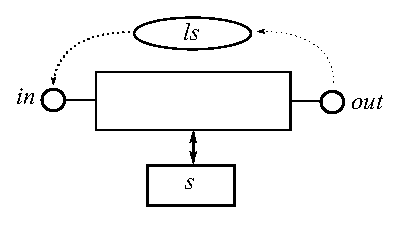
\includegraphics{images/atomic-action.eps}
%  \caption{Atomic Action view of the world}
%  \label{fig:atom-act:view}
%\end{figure}

\subsection{Atomic Action Semantics}

We use sets in two key ways:
checking for membership/subset inclusion;
and updating by simultaneously adding and removing elements:
%We use a shorthand (that views a set as its own collection
%of corresponding $n$-ary characteristic functions)
%as summarised in \figref{fig:short:membership}.
%The aim is to minimise displayed expression widths.
%\begin{figure}[t!]
%  \centering
%\begin{tabular}{|c|c|}
%\hline
%  Longhand & Shorthand
%\\\hline
%  $x \in S$ & $S(x)$
%\\\hline
%  $x \in \setof{y_1,\ldots,y_n} $ & $\setof{y_1,\ldots,y_n}(x)$
%\\\hline
%  $\setof{x_1,\ldots,x_n} \subseteq S$  & $S( x_1,\ldots,x_n)$
%\\\hline
%  $T \subseteq S$ & $S(T)$
%\\\hline
%  $\setof x$ &    $x$ (if context permits)
%\\\hline
%\end{tabular}
%  \caption{Set Membership Shorthands}
%  \label{fig:short:membership}
%\end{figure}
\RLEQNSs{
   A \ominus (B \rplby C) &\defs& (A \setminus B) \cup C
}
Let us consider an atomic state change operation,
viewed as a before-after relation on $State$:
\RLEQNSs{
   A(s,s') &:& State \rel State
}
We can lift this into an atomic concurrent action by adding in
the appropriate behaviour w.r.t to $in$, $out$, $ls$ and $ls'$:
\RLEQNSs{
    \A(A) &\defs& in \in ls \land A \land ls'=ls\ominus(\setof{in} \rplby\setof{out})
}
\noindent
To keep expression size manageable and clutter-free
we use a number of shorthands,
viz., $ls(in)$ for $ in \in ls$, $ls(a,b)$ for $\setof{a,b}\subseteq ls$,
$\ell$ for $\setof\ell$ (when it is clear a set is expected),
and $(a,b \rplby c,d)$ for ($\setof{a,b}\rplby \setof{c,d}$).
Given this shorthand we now write the atomic action semantics as:
\begin{equation*}
ls(in) \land A \land ls'=ls\ominus(in \rplby out)
\end{equation*}
A special case of this is the $Idle$ construct:
\RLEQNSs{
   Idle &\defs& \A(s'=s)
\\      &=& ls(in) \land s'=s \land ls'=ls\ominus(in \rplby out)
}
An atomic action has no need of the label generator $g$
so simply ignores it.
The situation with language composites is more complex, as we shall see.

\subsection{Composite Action Semantics}

For composite language constructs to work,
we require that the context of each component is somehow ``informed''
of how it is being situated.
We consider this the semantic responsibility of the composite itself,
and not something the components need to consider.

Let us consider sequential composition ($P \lseq Q$).
In effect, this operator has to glue its components
so that the $out$ label of the first corresponds to the $in$ label
of the second.
In effect it needs to generate a fresh label using $g$
and use this to replace the $out$ of $P$  and the $in$ of $Q$.
Then we need to split the generator in two and pass those bits
into $P$ and $Q$ for their own label generation needs.
The need for such generators arises because we can't use existential
quantification to hide a label,
because they need their presence in, or absence from, $ls$
to be globally visible.
We need these generators to have certain properties that ensure all
generated labels are unique,
and it is to this that we now turn.

\subsubsection{Label Generation}

We consider two operations that can be applied to a generator.
The first ($new$) returns a label, and a modified generator,
for further use.
The second ($split$) breaks a generator into two new generators
that will produce disjoint sets of labels.
To avoid long nested calls of $new$, $split$ and projections $\pi_1,\pi_2$,
we define the following terse label and generator expression syntax:
\RLEQNSs{
   g \in GVar && \text{Generator variables}
\\ G \in GExp &::=& g \mid G_{:} \mid G_1 \mid G_2
\\ L \in LExp &::=& \ell_G
}
Here $G_{:}$ denotes the generator left once $new$ has been run on $G$,
with $\ell_G$ denoting the label so generated.
Expressions $G_1$ and $G_2$ denote the two outcomes of applying $split$ to $G$.
We use $labs(G)$ to denote all the labels that $G$ can generate
and we require the following laws to hold:
\RLEQNSs{
   labs(G) &=& \setof{\ell_G} \cup labs(G_{:}) \cup labs(G_{1}) \cup labs(G_{2})
\\ \ell_G &\notin& labs(G_{:})
\\ \emptyset  &=& labs(G_{1}) \cap labs(G_{2})
}
The simplest model for a generator that satisfies the above constraints
is one that represents the label $\ell_G$ by the expression $G$ itself.
The reason for this shorthand is that without it we would have to write
something like the following
\begin{equation*}
\pi_1(new(\pi_2(new(\pi_2(split(\pi_2(new(\pi_1(split(g)))))))))).
\end{equation*}
instead of $\ell_{g1:2:}$.
%\begin{figure*}[t!]
%  \centering
%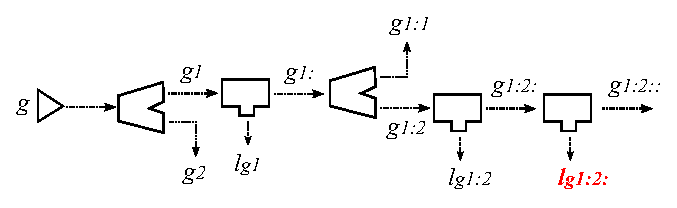
\includegraphics{images/label-gen-example.eps}
%  \caption{Label generation example: $\ell_{g1:2:}$}
%  \label{fig:label-gen-xampl}
%\end{figure*}
%(See \figref{fig:par-prog:view})

%\begin{figure}[t!]
%  \centering
%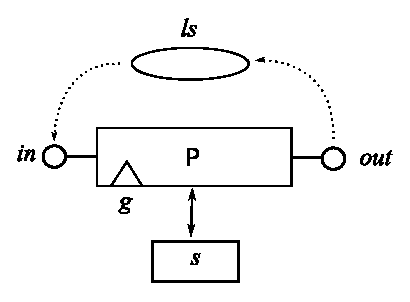
\includegraphics{images/parallel-program.eps}
%  \caption{Concurrent Program view of the world}
%  \label{fig:par-prog:view}
%\end{figure}


\subsubsection{Sequential Composition}





For sequential composition ($P \lseq Q$) we use the generator $g$
first to create the label ($\ell_g$) that connects $out$ of $P$ to $in$ of $Q$,
and then we split the leftover generator ($\g{:}$)
and give one ($\g{:1}$) to $P$, and the other ($\g{:2}$) to $Q$%
%(\figref{fig:seq-actual:view})
.
We simply use substitution to replace the static parameters
of both $P$ and $Q$ by the appropriate generator and label expressions.
\RLEQNSs{
    P \lseq Q &\defs& P[\g{:1},\ell_g/g,out] \lor Q[\g{:2},\ell_g/g,in]
}
We group the appropriately transformed components
using disjunction, as per the UTPP and action systems approach.
%\begin{figure*}[t!]
%  \centering
%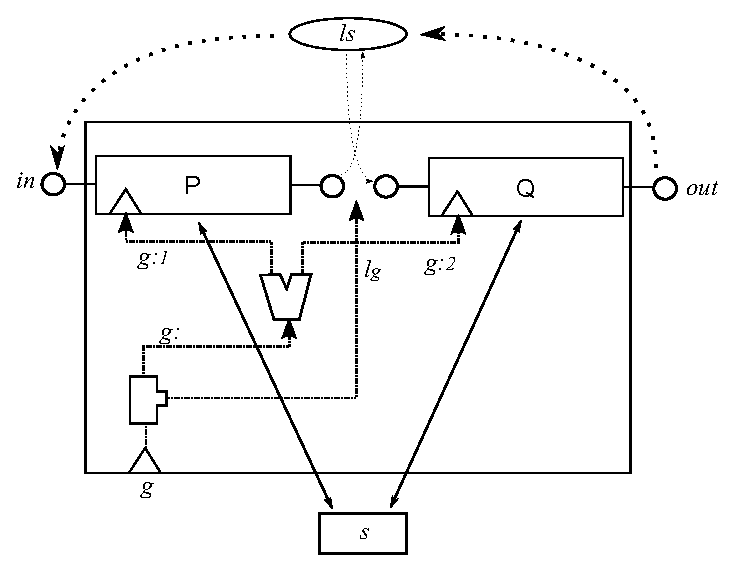
\includegraphics{images/seq-comp-actual.eps}
%  \caption{Sequential Composition actual construction}
%  \label{fig:seq-actual:view}
%\end{figure*}


\subsubsection{Parallel Composition}



Initially, parallel composition appears easy:
simply split the generator and pass to each part,
but leave $in$ and $out$ alone:
\[
  P[\g1/g] \lor Q[\g2/g]
\]
However this does not work---consider if $P$ is atomic and runs first:
the $in$ is removed from, and $out$ added to $ls$, effectively disabling $Q$.
Instead we need to seperate out the $in$ and $out$ labels of $P$ and $Q$,
and introduce two new atomic ``actions'': one to split $in$  into two new
start labels; and another to merge finish labels into $out$.
These split and merge actions do not alter state $s$.
We need to split the generator $g$ into two parts ($\g1,\g2$)
and generate two labels
(start: $\ell_{g1},\ell_{g2}$,
 finish: $\ell_{g1:},\ell_{g2:}$)
from each before passing them ($\g{1::},\g{2::}$) into $P$ and $Q$.
\RLEQNSs{
   Split(\ell_a,\ell_b)
   &\defs&
         ls(in)
   \land s'=s
   \land ls'=ls\ominus(in \rplby \ell_a,\ell_b)
\\ Merge(\ell_a,\ell_b)
   &\defs&
         ls(\ell_a,\ell_b)
   \land s'=s
\\ && {} \land ls'=ls\ominus(\ell_a,\ell_b \rplby out)
}
So, the parallel composition is a disjunction between
$Split(\ell_{g1},\ell_{g2})$,
the two components with appropriate re-labelling,
and $Merge(\ell_{g1:},\ell_{g2:})$%
%(\figref{fig:par-actual:view})
.
%\begin{figure}[t!]
%  \centering
%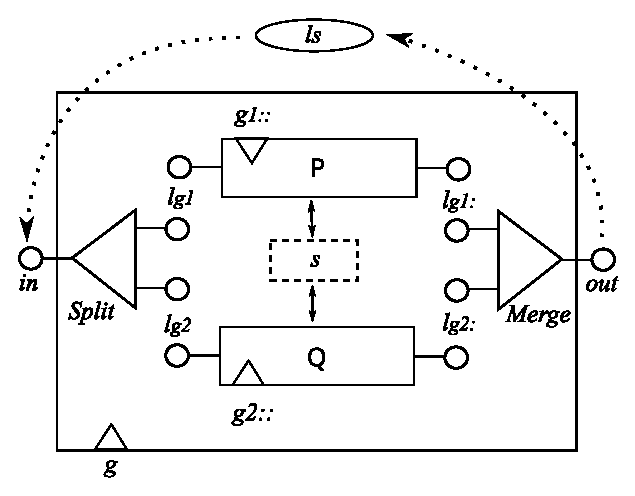
\includegraphics[scale=0.8]{images/par-comp-actual.eps}
%  \caption{
%     Parallel Composition actual construction (omitting generators).
%     The $s$ box is dashed to emphasise its global nature,
%     \emph{i.e.}, that it lies outside/under the program box
%  }
%  \label{fig:par-actual:view}
%\end{figure}
\RLEQNSs{
    P \parallel Q
    &\defs&
    ~~~~ Split(\ell_{g1},\ell_{g2})
\\&& {} \lor P[\g{1::},\ell_{g1},\ell_{g1:}/g,in,out]
\\&& {} \lor Q[\g{2::},\ell_{g2},\ell_{g2:}/g,in,out]
\\&& {} \lor Merge(\ell_{g1:},\ell_{g2:})
}

\subsubsection{Conditionals}

For the conditional, as only one arm will run, we can share $out$,
but we need a split on $in$ that uses the condition $c$.
\RLEQNSs{
   Cond(\ell_a,c,\ell_b)
   &\defs&
         ls(in)
   \land s'=s
\\ && {} \land ls'=ls\ominus(in \rplby \ell_a \cond c \ell_b)
}
So we split the generator $g$, yielding $\g1$ and $\g2$, and produce one start label from each
($\ell_{g1},\ell_{g2}$), and then pass the two remaining generators
($\g{1:},\g{2:}$)
into $P$ and $Q$ as appropriate.
We then have a conditional-split ``action'' that
converts $in$ into $\ell_{g1}$ or $\ell_{g2}$ as determined by the condition%
%(\figref{fig:cond-actual:view})
.
%\begin{figure}[t!]
%  \centering
%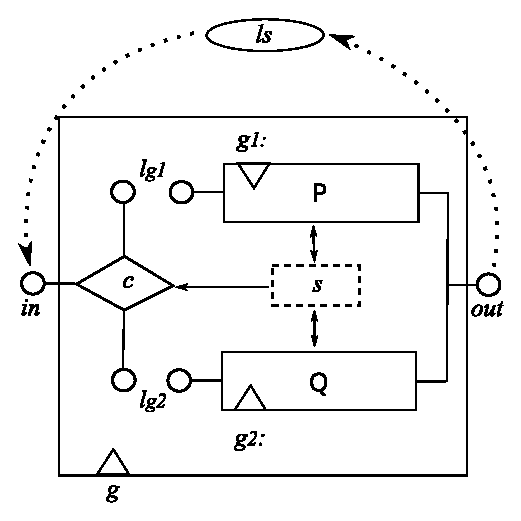
\includegraphics[scale=0.8]{images/conditional-actual.eps}
%  \caption{Conditional actual construction (omitting generators)}
%  \label{fig:cond-actual:view}
%\end{figure}
\RLEQNSs{
    P \lcond c Q
    &\defs& Cond(\ell_{g_1},c,\ell_{g2})
\\&& {} \lor P[\g{1:},\ell_{g1}/g,in] \lor Q[\g{2:},\ell_{g2}/g,in]
}

\subsubsection{Iteration}


Iteration is quite straightforward,
as we view it as a conditional loop unrolling%
%(\figref{fig:iter-actual:view})
.
We generate a label ($\ell_g$) for the entry-point to $P$,
pass the remaining generator ($\g:$) into $P$
and identify $P$'s exit with the loop entry.
%\begin{figure}[t!]
%  \centering
%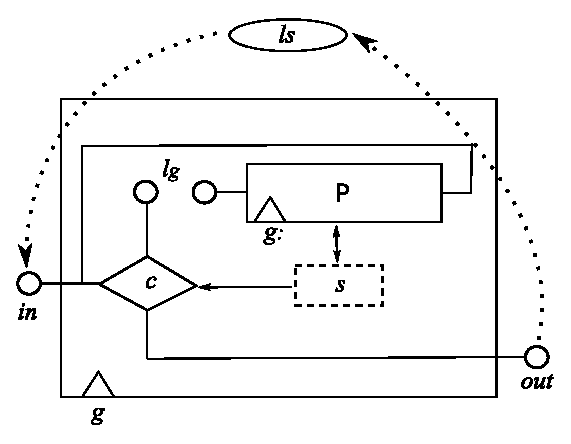
\includegraphics[scale=0.8]{images/iteration-actual.eps}
%  \caption{Iteration actual construction (omitting generators)}
%  \label{fig:iter-actual:view}
%\end{figure}
\RLEQNSs{
   c \wdo P
   &\defs&
    ls(in) \land s'=s \land ls'=ls\ominus(in \rplby \ell_{g} \cond c out)
\\&& {} \lor P[\g{:},\ell_{g},in/g,in,out]
}

\subsection{Running a concurrent program}

So far the semantics we have written simply views a concurrent program
as a big disjunction of atomic actions that use labels in a particular way.
This is a very static view of the program meaning.
To get a dynamic semantics we need to embed the above static
view, with appropriate initialisation,
into a loop that repeatedly runs the static disjunction
until a suitable (label-based) termination condition is reached.
We shall denote by $run(P)$ the result of adding dynamism
to a static view $P$ in this way.
We produce $run(P)$ by using the generator $g$
to create two labels $\ell_g$ and $\ell_{g:}$,
and then pass the remaining generator $\g{::}$
into the (static) program body $P$.
We use $\ell_g$ to replace $in$,
and $\ell_{g:}$ to replace $out$ in $P$.
We put this into a loop which keeps running so long as $\ell_{g:}$
is not in $ls$.
\RLEQNSs{
   run(P)
   &\defs&
   (\lnot ls(\ell_{g:}) * P[\g{::},\ell_{g},\ell_{g:}/g,in,out])[\ell_g/ls]
}
At the very top level, we initialise $ls$ to be $\setof{\ell_g}$.
Note that we cannot push this into the substitutions on $P$,
otherwise all that happens is that the first enabled action keeps running.

Space precludes us here from showing detailed calculations,
but we have obtained the following results which have
contributed to the validation of this semantics.
Here the lefthand side shows $P$, while the righthand side
shows a calculation of the expansion $run(P)$
\RLEQNSs{
   Idle
   &\stackrel{run}{\rightarrow}&
   s'=s \land ls'=\ell_{g:}
\\ \A(A)
   &\stackrel{run}{\rightarrow}&
   A \land ls'=\ell_{g:}
\\ \A(A) \lseq \A(B)
   &\stackrel{run}{\rightarrow}&
    ( A \seq B ) \land ls'=\ell_{g:}
\\ \A(A) \parallel \A(B)
   &\stackrel{run}{\rightarrow}&
    (( A \seq B ) \lor ( B \seq A))\land ls'=\ell_{g:}
\\ \A(A) \lcond c \A(B)
   &\stackrel{run}{\rightarrow}&
    ((c \land A ) \lor ( \lnot c \land B ))\land ls'=\ell_{g:}
}
Note that in each case we get a final result in terms of the
atomic actions on $s$ only,
plus an assertion that we have terminated.
For iteration we show a partial calculation
of $run(c \wdo \A(B))$ with result:
\RLEQNSs{
 && \lnot c \land s'=s
      \land ls'=\ell_{g:}
\\ &\lor&       c \land B \land \lnot c' \land ls'=\ell_{g:}
\\ &\lor& (~c \land B \land c' \land ls'=\ell_{g::}
\\ && \quad{};{} \A(B)[\g{:::},\ell_{g::},\ell_g,\ell_{g::}/g,in,out,ls]
\\ && \quad{};{} \lnot ls(\ell_{g:}) *
\\ && \qquad (c \wdo \A(B))
\\ && [\g{:::},\ell_{g::},\ell_g,\ell_{g::}/g,in,out,ls]
}
Here we see the result
of performing zero or one iteration, which also mentions only state,
plus a third case that captures the second and subsequent iterations.
In particular there is no mention in the final result of $in$ or $out$.

The semantics of $run(c \wdo \A(A))$ we expect to have a terminating part
and a non-terminating part:
\RLEQNSs{
 && (\bigvee_{i \in \Nat} A^i ) \land \lnot c \land ls'=\setof{\ell_{g:}}
       \lor A^\omega \land c \land \ell_{g:} \notin ls'
\\ \WHERE & & A^0 = s'=s
\\        & & A^{n+1} = A ; A^n
\\        & & A^\omega = \mbox{infinite sequence of $A$s}
}
From the above we can see that a possible interpretation of our semantics as a
Design is
\RLEQNSs{
   ok &\defs&  \ell_g \in ls
\\ ok' &\defs&  \ell_{g:} \in ls'
}
This works because every use of $run$ initialises $ls$ to $\ell_g$
and so establishes $ok$,
and the termination condition for $run$ is that $\ell_{g:}$
is has appeared in $ls$.
In fact the use of the generators ensures that, for all constructs,
that the labels $in$, $out$ and $labs(g)$ never occur together
in the label-set.

\HDRb{Healthiness Conditions}

Our semantics has been designed
to ensure that,
for any program $P$ with alphabet $s,s',ls,ls',in,out,g$,
during any program run,
the following four predicates
are mutually exclusive, and exhaustive:
\RLEQNS{
   (\setof{in,out}\cup lab(g)) \cap ls &=& \emptyset
                                    \label{eqn:asleep}
\\ in &\in& ls                      \label{eqn:just-started}
\\ lab(g) \cap ls &\neq& \emptyset  \label{eqn:running}
\\ out &\in& ls                     \label{eqn:just-stopped}
}
This observations comprise a key healthiness condition
that ensures that all  components get executed
in a coherent manner, moving from a ``sleeping state'' (\ref{eqn:asleep}),
to being just started (\ref{eqn:just-started}),
running (\ref{eqn:running}),
just finished (\ref{eqn:just-stopped}),
and then possibly back to being asleep.
We can accordingly define some program status predicates as follows:
\RLEQNSs{
   started(P)
   &\defs&
   in \in ls
\\ running(P)
   &\defs&
   \setof{in,out} \cap ls = \emptyset
   \land
   \exists \ell \in ls \bullet \ell \in labs(g)
\\ stopped(P) &\defs& out \in ls
}
Note that $running(\A(A))$ is always false,
as an atomic action effectively occurs instantly.

% \subsection{Bringing It All Together}\label{ha:unify}

We link the weak semantics to the UTCP version
by simply recognising that Weak PML simply views a PML description
as being the parallel composition of all its basic tasks.
We instantiate the generic state observation $s$
in the UTCP theory with the $r$ and $h$ observations of
the Weak theory, and define the semantics of a basic action $A$
as:
\RLEQNSs{
  N?rr!pr
  &\defs&
  rr \subseteq r \land \lnot pr \subseteq r
\\&& {} \land r' = r\cup rr \land h'= h \cat \seqof N
}
Here we drop $ok$ and $ok'$, as its role is subsumed by $ls$  and $ls'$
in the UTCP theory, and instead have a basic action return false when
its required resources are not available,
or all its provided resources
have been so provided.
%We can simply
%translate Weak PML to an equivalent Strong PML description
%by replacing every composite construct with parallel.
%\RLEQNSs{
%   W2S(A) &\defs& A
%\\ W2S(P \oplus Q)
%   &\defs& W2S(P) \parallel W2S(Q)
%   , \qquad \oplus\in\setof{\seq,\pcond,\parallel}
%\\ W2S(\piter P) &\defs& W2S(P)
%}
We note that when a PML description consists solely of basic tasks
and parallel composition, then the Weak, Flexible and Strict PML semantics
coincide since the control flow allows any task to run anytime,
so it is all just down to resource constraints.


%We can also circumvent the requirement for Weak PML task names to be unique
%by using the generator idea to create unique task labels
%which then form the domain of $\varpi$
%---we don't need any static parameters, as we just pass a generator
%in as an extra argument to $Coll$.

\subsection{Future Work}\label{ha:future}

One key issue we face in developing a strict or flexible semantics
is that the iteration construct has no explicit halting condition
associated with it syntactically.
The expectation is that an iteration is repeated until it brings
about a state of affairs that enables \emph{what comes after it}.
%In order to model this compositional,
%we need some way, in a sequential composition $P \seq Q$,
%for $Q$ to be able to signal back to $P$ that it has become ``enabled''.
%This has to be done without $P$ or $Q$ being aware of each others existence.
%This in turn requires that the establishment of that connection,
%between the enablement of $Q$
%and the stopping criterion of $P$ (if it is an iteration),
%has to be the responsibility of the $\seq$ constructor.
%The same notion of enablement can be used to allow the conditional
%construct to preferentially select for an enabled arm.
%
We believe that the UTP approach described in this paper will allow us
to produce a semantics that is compositional:
the iteration simply repeats until it gets a stop signal
sent by the enclosing sequential composition.

The instantiation of the flexible and strict semantics on top of UTCP
still has to be done,
as do the proofs regarding the laws of concurrent programs.
%A definitive list of these can be obtained by a careful reading
%of \cite{DBLP:journals/iandc/Brookes96}
%and consists of identities:
%\RLEQNSs{
%   P \lseq ( Q \lseq R) &=& ( P \lseq Q ) \lseq R
%\\ Idle \lseq P &=& P
%\\ P \lseq Idle &=& P
%\\ P \parallel Q &=& Q \parallel P
%\\ P \parallel ( Q \parallel R) &=& ( P \parallel Q ) \parallel R
%\\ P \parallel Idle &=& P
%\\ P \lcond{true} Q &=& P
%\\ P \lcond{false} Q &=& Q
%\\ (P \lcond c Q) \lseq R &=& (P \lseq R) \lcond c (Q \lseq R)
%\\ c \wdo P &=& (P \lseq c \wdo P) \lcond c Idle
%}
%and refinements:
%\RLEQNSs{
%   P \lseq Q &\refinedby& P \parallel Q
%\\ P \lseq (Q \parallel R) &\refinedby& (P \lseq Q) \parallel R
%\\ P \lcond{c_1 \land c_2} Q &\refinedby&
%   (P \lcond{c_2} Q) \lcond{c_1} Q
%}
The proof sketches done so far show indicate that
the proofs will require demonstrating the existence
of label bijections that respect control-flow,
and that a benefit of constructing such bijections
will be a corresponding operational semantics for UTCP.

We are also working on ideas for a variant of UTCP
that shows promise for being fully compositional:
\emph{i.e.}, without having a static disjunction
of actions, that then needs something like $run$
to make it all dynamic.
We also point out, in the spirit of unification,
that this work has potential to go beyond just PML
but also assist in the development of other theories
of concurrency in UTP,
such as pioneering work in \cite{journals/fac/ZhuHQB15}
addressing the semantics of System-C.

We prefer the UTP denotational/algebraic approach
to that of using operational semantics.
The former typically requires redoing induction proofs
when any change is made,
whereas adding new features and merging models is
much simpler with the latter\cite[p277]{Hoare-He98}.

% \section{Related Work}\label{ha:related}


\subsection{Process Semantics}

Our motivation for wanting to formalise PML
comes from its applicability in modelling clinical healthcare pathways
\cite{Campbell98}
in particular,
as well as its use to model certified medical software development processes.
Clinical pathways are evidence-based care plans which describe in a
structured way the essential steps needed to care for patients with a
specific set of clinical problems.





Formalisms that model CPs, need to be able to 'reason' with process behaviour
such as non-determinism, concurrency, parallelism and synchronisation. The
affinity of the Petri nets formalism to represent such behaviour has
contributed to its popularity to be used in the more 'formal spectrum' of CPs
research. Petri nets have been used to model such work-flows
\cite{Ellis95,vanderAalst96,Eshuis03}.
Stochastic treatments are popular
for looking at resource and time estimation, e.g. ICPA\cite{Yang12}.

A key issue with any attempt to model such pathways is the need
to allow flexibility in how they are actually implemented.
Work by van der Aalst et al \cite{vanderAalst06} proposes an approach (based on Petri
nets) to allow the ability to distinguish between
 marginally different and completely different processes.
Work looking for temporal similarity
using ad hoc temporal constraint networks,
has been reported in \cite{Combi09}.
Other approaches include the use of fuzzy logic \cite{Adam05}
or linear temporal logic expressions \cite{Pesic06}.
Of interest is the work of Grigori et al \cite{Grigori01}
that use the concept of anticipation which allows
the execution of sequential tasks to overlap at the discretion of work-flow
users where there are not specific data dependencies between them.

Some interesting recent work using BPMN\cite{DBLP:conf/caise/GiacomoDMM15}
addresses the same issue that we do,
namely being able to be flexible regarding how models get enacted.
This paper looks at the boundary between strict imperative BPMN
and declarative notations such as Declare\cite{DBLP:conf/edoc/PesicSA07}.
These correspond to our Strict and Weak semantics.
They introduce BPMN-D and give its semantics by translation
to plain BPMN, whose semanitcs is based on Petri-Nets\cite{DBLP:journals/infsof/DijkmanDO08}.


\subsection{Concurrency Semantics}

Key work was done on concurrent semantics in the 80s and 90s,
with a strong focus on fully abstract denotational
semantics.
Notable work form this period includes that by
Stephen Brookes\cite{DBLP:journals/iandc/Brookes96}
and Frank de Boer and colleagues\cite{DBLP:conf/concur/BoerKPR91}.
Both looked at denotations based on the notion of sets of transition traces,
these being sequences of pairs of before-after states.
In order to get compositionality the traces of any program fragment
had to have arbitrary ``stuttering'' and ``mumbling'' state-pairs
added to capture the notion of outside interference.
Full abstraction meant that the semantics had to identify
programs like $skip\lseq skip$ with $skip$,
while distinguishing between $x:=2$ and $x:=1\lseq x:=x+1$.
This latter aspect required the language to be augmented with
an atomic wrapper construct.
A common feature of both was the very close linkage of the denotational
semantics to the operational one.
The work of Brookes\cite{DBLP:journals/iandc/Brookes96}
focussed on imperative languages with fair schedulers,
while that of de Boer et.al\cite{DBLP:conf/concur/BoerKPR91}
looked at a general framework (``failures of failures'')
that covered not just imperative programs
but also constraint solving systems
and \emph{asynchronous} versions of process algebras.


As already stated earlier,
the key inspiration and starting point for the work presented here
was the UTPP paper\cite{DBLP:conf/icfem/WoodcockH02}.
This combined guarded commands\cite{1976:book:dijkstra}
with the idea of action systems\cite{PODC::BackK1983},
interpreted in UTP as non-deterministic choice
over guarded atomic actions,
where disabled actions behave like the unit for that choice.
This basic lattice-theoretic architecture for the UTPP semantics
forms the foundation for the UTCP semantics presented here.

% \section{Conclusions \& Future Work}\label{ha:conc}


We have briefly described Process Modelling Language (PML)
that is used to model business processes,
with clinical pathways being an interesting specific case,
with a view to defining formal semantics for the notation
that allows rigorous reasoning in a flexible manner.
This need arises because clinical pathways in real medical practise
are often interpreted in a loose manner,
although also intended to be quite prescriptive.
%A common issue that arises is that an experienced medic
%might enact such a pathway in a very flexible manner,
%based on their experience, while a junior doctor would be expected,
%and advised, to stick the described protocol far more closely.

We have presented a UTP theory of a ``weak'' interpretation
of PML,
as well as a UTCP theory of concurrency that
acts as a baseline theory on top of which the ``flexible''
and ``strict'' interpretations may be constructed.
A key contribution here is the use of label generators
and the distinction between dynamic state-change observables,
and static context-sensitive parameters.

One other benefit of using the UTP framework here
is that it will ease the integration of application-specific
resource semantic models,
so that we can envisage complete formal analyses
that address application area concerns,
e.g. drug interactions in clinical pathways.





\end{document}
